\chapter{Java静态安全扫描工具需求分析与设计}
\section{系统整体概述}
Java语言通常用于Web服务和Android程序开发,其中的大量安全漏洞类型可以通过污点传播分析法进行扫描,然而随着漏洞种类和开发方式不断丰富,污点分析存在失误,因此产生了大量误报,为此安全工程师不得不修改污点传播规则,以增加漏报为代价换取低误报,或是人工对大量误报漏洞判断,这两种做法无疑会增加潜在安全风险。

本系统旨在提供对于Java代码的更精确的漏洞静态扫描功能,在源代码开发阶段进行代码安全扫描。相对于传统污点传播扫描工具,本系统结合了程序切片和BLSTM,从已有的误报漏洞片段进行分析,降低污点传播误报率。系统总体架构如图~\ref{overview}所示,系统主要分为前端和后端两大部分,前端部分运行在用户端,包含污点分析模块、程序切片模块、部分预测模块,而在扫描系统后端运行在服务器端,包含预处理模块,另一部分预测模块和数据库。

污点分析模块对开源的find-sec-bugs做改进,使之能够输出污点传播树,为误报预测提供基础数据;程序切片模块分析污点传播树,将其拆分为子污点传播流,利用Joana生成SDG并进行切片;数据预处理模块将切片模块的输出数据进行泛化和向量化处理,使之可以输出预测模块;误报预测模块利用切片模块的子污点传播流和其对应切片,通过BLSTM进行切片预测,从而对漏洞进行预测。本系统采用客户端采用Java进行开发,管理后台和程序预测服务由Python和Django开发。

\begin{figure}[htb]
	\centering
	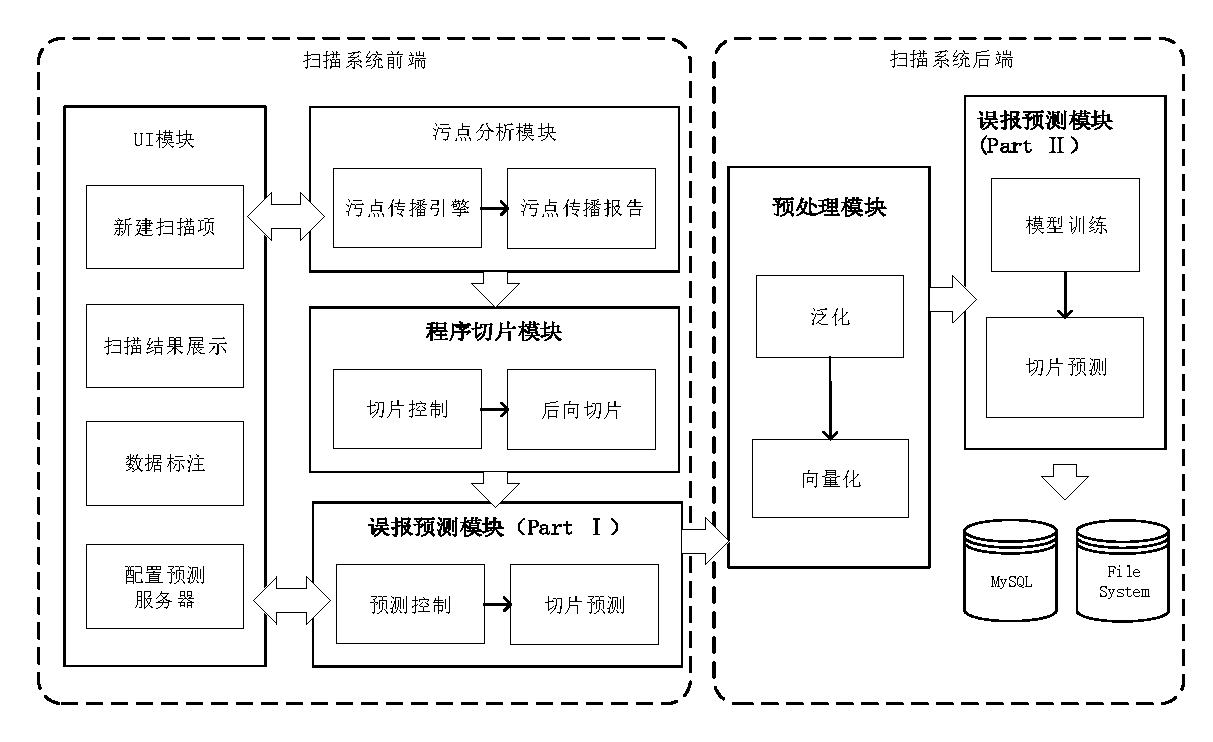
\includegraphics[width=5in]{FIGs/chapter3/system-architecture.pdf}
	\caption{系统总体架构图}\label{overview}
\end{figure}

\section{系统需求分析}\label{sec:demand}
\subsection{功能性需求}
本系统功能性需求分析按污点分析模块,程序切片模块,预处理模块和误报预测模块四个方面进行。

污点分析模块由污点分析引擎对用户提交的jar文件进行扫描,产生初步结果,该模块所涉及的功能性需求如表~\ref{dmd:taint}所示,其主要功能为污点分析,而对于用户来说,系统需要友好的展现污点分析结果,即存在构造污点传播树和查看分析结果的需求,污点传播树由污点传播图构造而来,因此存在构造污点传播图需求,此外,污点分析是一项耗时操作,用户(尤其是开发工程师)可能会对一次污点分析结果进行保存,交给安全工程师进行漏洞验证,因此系统最好还需有保存分析结果和读取分析结果功能。

\begin{table}[!htbp]\footnotesize %label table
	\centering
	\caption{污点分析模块功能性需求列表}
	\vspace{2mm}
	% l - left, r - right, c - center. | means one vertical line 这里声明的是表格单元中的内容如何对齐
	\begin{tabular}{L{1.3cm}L{2.5cm}L{6.8cm}L{1.5cm}}
		\toprule
		\textbf{需求编号}&\textbf{需求名称}&\textbf{需求内容}&\textbf{优先级}\\
		\midrule
		R1	& 污点分析 				& 对于用户上传的代码进行污点分析,包括了过程内分析和过程间分析 & 高 \\
		R2  & 构造污点传播图 	 & 对于代码中存在的汇聚点,构造其污点传播图 & 高 \\
		R3  & 构造污点传播树	 & 对于一个污点传播类型的分析结果,用户最终看到一棵或多课污点传播树,其由污点传播图构造,一张污点传播图可能有多棵传播树,一个传播树上清晰标注有一个产生点和一个汇聚点 & 高 \\
		R4  & 查看分析结果	 & 对于一个污点传播类型的分析结果,用户最终看到一棵或多课污点传播树,对于树上的叶子节点,用户能够知晓其代码位置 & 高 \\
		R5  & 保存分析结果	   &用户可以对当前代码的漏洞分析详情进行保存,其中关键点在于对污点传播树进行序列化 & 中 \\
		R6  & 读取分析结果 	   &用户可以对保存后的分析结果文件进行读取,二次查看漏洞详情,其中关键点在于对污点传播树结构的反序列化 & 中 \\
		\bottomrule
	\end{tabular}
	\label{dmd:taint}
\end{table}

程序切片模块对污点分析结果进行切片处理,该模块所涉及的功能性需求如表~\ref{dmd:slice}所示,该模块的主要功能是根据污点分析模块的分析结果进行后向程序切片,将其拆解,得到四个子需求,首先其需要污点分析的结果进行处理,接着对污点传播树进行拆分,对于每一个污点传播流,其包含有若干个子污染流,下一步对这些需求进行后向切片,最后将切片结果转换为有一定结构的文本。

\begin{table}[!htbp]\footnotesize %label table
	\centering
	\caption{程序切片模块功能性需求列表}
	\vspace{2mm}
	% l - left, r - right, c - center. | means one vertical line 这里声明的是表格单元中的内容如何对齐
	\begin{tabular}{L{1.3cm}L{2.5cm}L{6.8cm}L{1.5cm}}
		\toprule
		\textbf{需求编号}&\textbf{需求名称}&\textbf{需求内容}&\textbf{优先级}\\
		\midrule
		R7	 & 处理污点分析结果 & 对污点分析的结果进行处理,对于每一个漏洞实例,反序列化的污点传播树 & 高 \\
		R8	 & 污点传播树拆分 & 将每一个传播树拆分为多个子污点传播流,每一个污点传播流包含若干个<函数入口点,关注点>对(其为一个切片的单位) & 高 \\
		R9   & 后向程序切片 & 对于每一个<函数入口点,关注点>, 结合用户上传的Jar包,进行后向程序切片 & 高 \\
		R10 & 输出切片结果	 & 对于切片,程序能将其表示为文本,即对切片结构体序列化 & 高 \\
		\bottomrule
	\end{tabular}
	\label{dmd:slice}
\end{table}

预处理模块对切片结果进行预处理,该模块所涉及的功能性需求如表~\ref{dmd:preprocessing}所示,该模块的主要功能是对切片文本进行泛化和向量化,在泛化需求主要保证一个切片能代表一类代码片段;随后进行向量化,对于切片的单词序列进行token标记,从而产生字典和切片向量,即BLSTM模型的输入。此外,一个较低优先级的需求为根据字典,将切片向量还原为切片的单词序列。

\begin{table}[!htbp]\footnotesize %label table
	\centering
	\caption{预处理模块功能性需求列表}
	\vspace{2mm}
	% l - left, r - right, c - center. | means one vertical line 这里声明的是表格单元中的内容如何对齐
	\begin{tabular}{L{1.3cm}L{2.5cm}L{6.8cm}L{1.5cm}}
		\toprule
		\textbf{需求编号}&\textbf{需求名称}&\textbf{需求内容}&\textbf{优先级}\\
		\midrule
		R11   & 泛化 & 对于每一个切片进行泛化处理,包括抽象数值、字符串、类名和方法名等 & 高 \\
		R12 & 向量化	 & 对于一个切片的单词序列,生成单词与整形值的字典并按字典对其向量化 & 高 \\
		R13 & 反向量化	 & 对于一个单词序列的向量,根据字典将其还原为切片的单词序列 & 低 \\
		\bottomrule
	\end{tabular}
	\label{dmd:preprocessing}
\end{table}

误报预测模块是对保障漏洞报告准确性的核心模块,包括客户端、后端和Web前端部分,该模块所涉及的功能性需求如表~\ref{dmd:predict}所示,该模块的需求主要为对给定漏洞实例进行预测,标记以及模型训练。预测依赖后端服务,因此有设置后端服务器的需求;预测分为预测切片安全性需求和预测漏洞真实性需求,分别由后端服务和客户端实现;标记分为对切片安全性标记和漏洞真实性标记,当漏洞标记为误报时,用户需指定安全的污染流;同时,管理员有训练预测模型的需求;此外,由于预测过程并不是很占用资源,对保存预测结果的需求程度较低;最后用户可以清空标记和预测结果。

\begin{table}[!htbp]\footnotesize %label table
	\centering
	\caption{误报预测模块功能性需求列表}
	\vspace{2mm}
	% l - left, r - right, c - center. | means one vertical line 这里声明的是表格单元中的内容如何对齐
	\begin{tabular}{L{1.3cm}L{2.5cm}L{6.8cm}L{1.5cm}}
		\toprule
		\textbf{需求编号}&\textbf{需求名称}&\textbf{需求内容}&\textbf{优先级}\\
		\midrule
		R14 & 预测切片安全性 & 对于一个切片向量,预测该切片是否是安全的(污染流无法传播) & 高 \\
		R15 & 标记切片安全性	 & 对切片向量,标记其是否安全 & 高 \\
		R16 & 预测漏洞真实性 & 用户在客户端可以查看预测结果,即该漏洞是否真实存在,需要结合切片预测需求 & 高 \\
		R17 & 标记漏洞真实性	 & 用户在客户端可以对于一个漏洞,标记漏洞是否存在,不存在时用户需提供理由(指出安全的污染流) & 高 \\
		R18 & 训练预测模型	 & 管理员可以在Web页面发起训练模型任务,或是安排定时器定期更新模型 & 高 \\
		R19 & 保存预测结果	 & 用户在客户端可以保存漏洞预测结果 & 低 \\
		R20 & 清空标记和预测结果	 & 用户在客户端可以清空标记和预测结果,以便重新预测 & 低 \\
		R21 & 设置预测服务器	 & 用户在客户端设置远程服务器 & 中 \\
		\bottomrule
	\end{tabular}
	\label{dmd:predict}
\end{table}


\subsection{非功能性需求}
本系统旨在为开发者和安全工程师提供Java代码安全扫描功能,考虑到系统功能性质、使用场景和所属领域,系统的非功能性需求主要有高效率,健壮性,保密性,安全性和扩展性五点。

首先,本系统的功能点在于对Java代码进行安全扫描,其使用场景位于软件开发至测试阶段,因此扫描过程要保证一定的效率和健壮性,如果一次扫描等待时间过长,或是扫描过程中途崩溃,那么开发过程就会受到影响,甚至影响整个服务的可用性,因此本系统需要是高效且健壮的。

其次,本系统涉及软件安全领域,很可能是恶意攻击者的首要攻击对象,因此自身需要具备保密性和安全性,这里的保密性是指保证用户提交的Java代码和Jar包的数据安全,安全性是指扫描服务本身经过充分安全性测试,不出现安全漏洞。

最后,很多企业目前已经拥有了适用于自身特点的基于污点传播的扫描器,为此,系统需要保证一定的扩展性,如将污点传播的解析抽象为接口,保证其可以基于任意污点传播工具进行预测。\\

\subsection{系统用例描述}\label{sec:case}
%用例图
本系统的主要用户为软件开发工程师和软件安全运营人员,根据对系统需求的分析,得到系统用例如图~\ref{fig:case}所示, 软件开发工程师和运营人员均有基于污点分析的静态扫描、扫描结果切片和预测、漏洞实例标记这三个用例,其中基于污点分析的静态扫描存在两例扩展用例,即保存污点分析结果和读取分析结果,漏洞实例标记实际包含了标记正报结果和标记误报结果用例,安全运营人员还多出模型训练和发放客户端口令的用例。

\begin{figure}[!htbp]
	\centering
	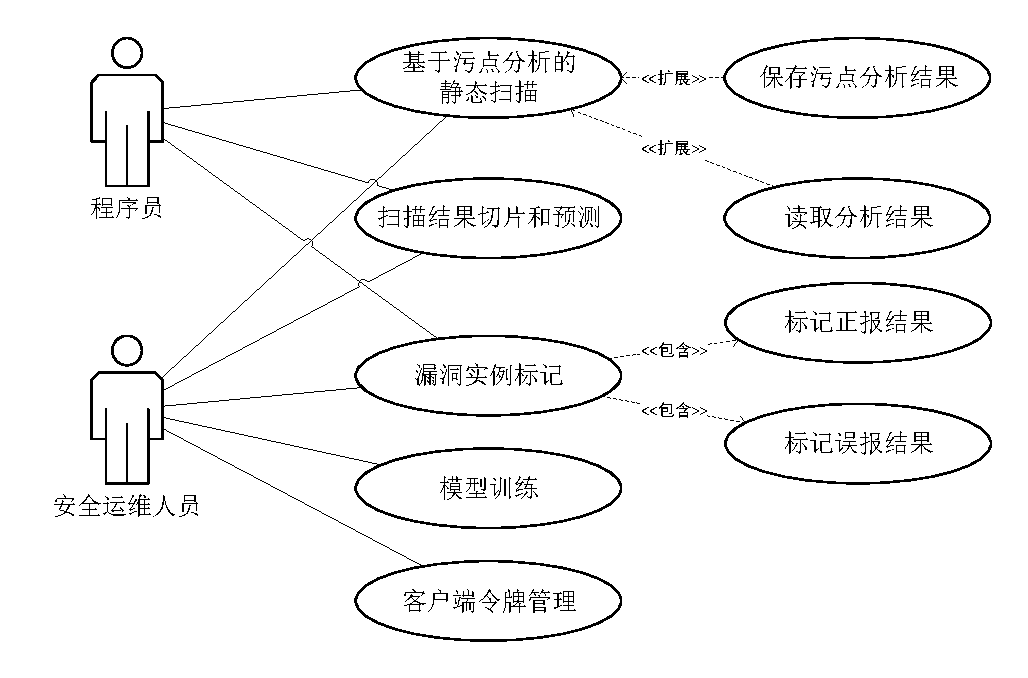
\includegraphics[width=5in]{FIGs/chapter3/case.pdf}
	\caption{系统用例图}\label{fig:case}
\end{figure}

\newcounter{caseCounter}
\setcounter{caseCounter}{1}

基于污点分析进行程序的静态扫描是本系统的基本功能,同样也是漏洞预测的基础。其用例描述如表~\ref{case:taint}所示,安全工程师或软件工程师(下面统称“用户”)对将开发好的项目进行构建,新建项目时将源代码和构建得到的Jar/War包添加到项目中,随后系统对其进行污点分析,并返回给用户潜在的安全漏洞。
% 1基于污点分析的静态扫描
\begin{table}[!htb]\footnotesize %label table
	\centering
	\caption{基于污点分析的静态扫描用例描述}
	\vspace{2mm}
	% l - left, r - right, c - center. | means one vertical line 这里声明的是表格单元中的内容如何对齐
	\begin{tabular}{L{3cm}L{10cm}}
		\toprule
		\textbf{描述项}&\textbf{说明}\\
		\midrule
		用例编号 & C\arabic{caseCounter}\stepcounter{caseCounter} \\
		用例名称 & 基于污点分析的静态扫描用例 \\
		对应功能需求编号  & R1, R2, R3, R4 \\ 
		参与者 & 用户 \\
		前置条件 & 用户已开发好项目并已构建的Jar/War包 \\
		后置条件 & 无\\
		正常流程 & \tabincell{l}{
							1. 用户选择“文件”,“新建项目”,打开新建项目会话框\\
							2. 用户输入项目名称,选择需要分析的包文件以及源文件所在目录\\
							3. 用户点击“分析”按钮,程序开始对其进行基于污点分析的静态扫描\\
							4. 用户在界面上看到漏洞列表,点击一个污点传播类型的漏洞\\
							5. 用户在界面上看到该漏洞的污点传播树\\
							6. 用户点击任意污点传播树的叶子节点,在界面上看到对应的源代码
					}\\
		异常流程 & 2. 若出现异常,则弹出异常会话框并显示异常信息\\
		\bottomrule
	\end{tabular}
	\label{case:taint}
\end{table}

% 2保存分析结果
污点分析后,用户可以对其分析结果进行保存,其用例描述见表~\ref{case:taintsave},用户点击保存按钮后,系统将污点传播树的每一节点序列化漏洞注解,并将含有一组注解的一系列漏洞保存为本地文件。

\begin{table}[!htb]\footnotesize %label table
	\centering
	\caption{保存污点分析结果用例描述}
	\vspace{2mm}
	% l - left, r - right, c - center. | means one vertical line 这里声明的是表格单元中的内容如何对齐
	\begin{tabular}{L{3cm}L{10cm}}
		\toprule
		\textbf{描述项}&\textbf{说明}\\
		\midrule
		用例编号 & C\arabic{caseCounter}\stepcounter{caseCounter}  \\
		用例名称 & 保存污点分析结果用例 \\
		对应功能需求编号  & R5 \\ 
		参与者 & 用户  \\
		前置条件 & 用户已创建项目且进行了基于污点分析的静态扫描 \\
		后置条件 & 用户指定位置出现保存好的分析报告\\
		正常流程 & \tabincell{l}{
			1. 用户选择“文件”,“另存为”,打开另存为对话框\\
			2. 用户输入保存文件名、文件类型和保存位置,点击保存按钮,分析结果\\被保存
		}\\
		异常流程 & 2. 若出现异常,则弹出异常会话框并显示异常信息\\
		\bottomrule
	\end{tabular}
	\label{case:taintsave}
\end{table}

% 3读取分析结果
对于以保存的分析结果,用户可以加载它们重新分析漏洞结果,程序对分析结果反序列化后在界面显示先前分析结果,如表~\ref{case:taintload}所示。

\begin{table}[!htb]\footnotesize %label table
	\centering
	\caption{读取分析结果用例描述}
	\vspace{2mm}
	% l - left, r - right, c - center. | means one vertical line 这里声明的是表格单元中的内容如何对齐
	\begin{tabular}{L{3cm}L{10cm}}
		\toprule
		\textbf{描述项}&\textbf{说明}\\
		\midrule
		用例编号 & C\arabic{caseCounter}\stepcounter{caseCounter}  \\
		用例名称 & 读取分析结果用例 \\
		对应功能需求编号  & R6 \\ 
		参与者 & 用户  \\
		前置条件 & 用户磁盘中已有一份污点分析报告 \\
		后置条件 & 无\\
		正常流程 & \tabincell{l}{
			1. 用户选择“文件”,“打开”,显示打开文件对话框\\
			2. 用户在打开文件对话框中选择报告文件,点击“打开”按钮,程序\\加载并在界面上显示污点分析报告中的内容
		}\\
		异常流程 & 2. 若出现异常,则弹出异常会话框并显示异常信息息\\
		\bottomrule
	\end{tabular}
	\label{case:taintload}
\end{table}

% 4设置预测服务器
对于客户端来说,对漏洞进行标记或者预测前提需要设置远程服务器,设置预测服务器的用例描述如表~\ref{case:setserver}所示,用户通过管理员发放的token和服务器地址设置远端服务器。
\begin{table}[!htb]\footnotesize %label table
	\centering
	\caption{设置预测服务器用例描述}
	\vspace{2mm}
	% l - left, r - right, c - center. | means one vertical line 这里声明的是表格单元中的内容如何对齐
	\begin{tabular}{L{3cm}L{10cm}}
		\toprule
		\textbf{描述项}&\textbf{说明}\\
		\midrule
		用例编号 & C\arabic{caseCounter}\stepcounter{caseCounter}  \\
		用例名称 & 设置预测服务器用例 \\
		对应功能需求编号  & R21 \\ 
		参与者 & 用户  \\
		前置条件 & 管理员已向用户发放token \\
		后置条件 & 无\\
		正常流程 & \tabincell{l}{
			1. 用户选择“AI”,“Set Server”,显示服务器设置对话框\\
			2. 用户服务器对话框汇中设置服务器地址以及token信息\\
			3. 用户点击“验证”按钮,检查配置是否正确\\
			4. 用户点击“应用”按钮,完成服务器配置
		}\\
		异常流程 & 2. 若出现异常,则弹出异常会话框并显示异常信息\\
		\bottomrule
	\end{tabular}
	\label{case:setserver}
\end{table}

% 5扫描结果预测
扫描结果切片和预测功能是本系统的最核心功能,程序首先对污点传播结果分析,拆解为污点传播片段并分别切片,再由服务端预测每一个切片是否为清洁片段,最后得出漏洞实例是否为真实漏洞。涉及的用例描述如表~\ref{case:predict}所示。

\begin{table}[!htbp]\footnotesize %label table
	\centering
	\caption{扫描结果切片和预测用例描述}
	\vspace{2mm}
	% l - left, r - right, c - center. | means one vertical line 这里声明的是表格单元中的内容如何对齐
	\begin{tabular}{L{3cm}L{10cm}}
		\toprule
		\textbf{描述项}&\textbf{说明}\\
		\midrule
		用例编号 & C\arabic{caseCounter}\stepcounter{caseCounter}  \\
		用例名称 & 扫描结果切片和预测用例 \\
		对应功能需求编号  & R7, R8, R9, R10, R14, R16 \\ 
		参与者 & 用户  \\
		前置条件 & 用户已完成远程服务器配置并且已有污点分析结果 \\
		后置条件 & 预测所需所有切片信息发送至服务器\\
		正常流程 & \tabincell{l}{
			1. 用户选择“AI”点击“Slice and Predict”,程序开始对污点分析结\\果进行切片和预测\\
			2. 用户等待切片和预测完成时,可以在弹出的会话框中观察预测进度,\\并随时取消预测\\
			3. 用户在程序主界面看到每一漏洞预测结果,预测为误报的漏洞由灰色\\图标标识且在漏洞列表标注为“(P: FP)”,预测结果为正报的漏洞图标\\不变,文字标注为“(P: TP)”\\
			4. 用户在点击一个漏洞,在污点传播图上可以看到预测解释,当预测结果\\为误报时,所有与预测为安全的污点传播流相关的叶子节点由“(*)”标\\注。
		}\\
		异常流程 & 2. 若出现异常,则弹出异常会话框并显示异常信息\\
		\bottomrule
	\end{tabular}
	\label{case:predict}
\end{table}

% 6标记正报结果
预测模块的学习模型为监督式学习模型,因此对漏洞报告结果进行标记是预测准确性提升的关键,在实际应用时,即使没有学习模块,开发者或是安全工程师也会对漏洞报告进行是否为误报的判断,因此本系统只是利用了用户的反馈使其构成回路,而并没有加重用户的使用负担。若漏洞实例被安全工程师判断为真实存在的,工程师可以对该漏洞标记为正报,此时所有污染流片段均自动标记为不安全,并且发送给服务端。标记正报结果用例描述如表~\ref{case:labeltp}所示。

\begin{table}[!htbp]\footnotesize %label table
	\centering
	\caption{标记正报结果用例描述}
	\vspace{2mm}
	% l - left, r - right, c - center. | means one vertical line 这里声明的是表格单元中的内容如何对齐
	\begin{tabular}{L{3cm}L{10cm}}
		\toprule
		\textbf{描述项}&\textbf{说明}\\
		\midrule
		用例编号 & C\arabic{caseCounter}\stepcounter{caseCounter}  \\
		用例名称 & 标记正报结果用例 \\
		对应功能需求编号  & R15, R17 \\ 
		参与者 & 用户  \\
		前置条件 & 用户已经对污点分析结果进行了切片和预测 \\
		后置条件 & 用户指定漏洞的所有污染流片段均标记为不安全且发送至服务器\\
		正常流程 & \tabincell{l}{
			1. 用户右键点击需要标记的正报漏洞实例,弹出标记菜单\\
			2. 用户点击“Labeled as True Positive”,该漏洞被标记为正报,漏洞说\\明内容被显示为“[L: TP]”
		}\\
		异常流程 & 2. 若出现异常,则弹出异常会话框并显示异常信息\\
		\bottomrule
	\end{tabular}
	\label{case:labeltp}
\end{table}

% 7标记误报结果
若漏洞实例被用户判断为不存在,用户可以对该漏洞标记为误报,此时用户需要指定一条最短的污染流,并且在该污染流中污点消失,同时,这段“安全的污染流”被发送至服务端。标记误报结果用例描述如表~\ref{case:labelfp}所示。

\begin{table}[!htb]\footnotesize %label table
	\centering
	\caption{标记误报结果用例描述}
	\vspace{2mm}
	% l - left, r - right, c - center. | means one vertical line 这里声明的是表格单元中的内容如何对齐
	\begin{tabular}{L{3cm}L{10cm}}
		\toprule
		\textbf{描述项}&\textbf{说明}\\
		\midrule
		用例编号 & C\arabic{caseCounter}\stepcounter{caseCounter}  \\
		用例名称 & 标记误报结果用例 \\
		对应功能需求编号  &  R15, R17 \\ 
		参与者 & 用户  \\
		前置条件 & 用户已经对污点分析结果进行了切片、预测或标记 \\
		后置条件 & 无\\
		正常流程 & \tabincell{l}{
			1. 用户右键点击需要标记的误报漏洞实例,弹出标记菜单\\
			2. 用户点击“Labeled Safe Flow”,弹出误报标记会话框\\
			3. 用户选择一条最短的安全污染流,同时看到该污染流的哈希和切片信\\息,点击确定后完成标记\\
			4. 用户看到其所标记的漏洞被标注为“[L: FP]”,并且在污染传播树中,\\所有与被用户标记的那段污染流相关的叶子节点由“[*]”标记。
		}\\
		异常流程 & 2. 若出现异常,则弹出异常会话框并显示异常信息\\
		\bottomrule
	\end{tabular}
	\label{case:labelfp}
\end{table}

% 8清空切片、标记和预测结果
由于切片、预测是复杂操作,系统会将其放入缓存,同时标记结果用户也会有想清空的情况,因此本系统提供一键清除切片、标记和预测结果的功能。其用例描述如表~\ref{case:clean}所示。
\begin{table}[!htb]\footnotesize %label table
	\centering
	\caption{清空切片、标记和预测结果用例描述}
	\vspace{2mm}
	% l - left, r - right, c - center. | means one vertical line 这里声明的是表格单元中的内容如何对齐
	\begin{tabular}{L{3cm}L{10cm}}
		\toprule
		\textbf{描述项}&\textbf{说明}\\
		\midrule
		用例编号 & C\arabic{caseCounter}\stepcounter{caseCounter}  \\
		用例名称 & 清空切片、标记和预测结果用例 \\
		对应功能需求编号  & R20 \\ 
		参与者 & 用户  \\
				前置条件 & 用户已经对污点分析结果进行了切片和预测 \\
		后置条件 & 用户指定漏洞的最短安全污染流被标记为安全且发送至服务器\\
		正常流程 & \tabincell{l}{
			1. 用户选择“AI”点击“Clean DB”,程序清空切片、预测和标记数据,\\并在漏洞的预测标签上显示“(P: UNK)”,在标记标签上显示“[L: UNK]”
		}\\
		异常流程 & 无\\
		\bottomrule
	\end{tabular}
	\label{case:clean}
\end{table}

% 9模型训练
模型训练的用例描述如表~\ref{case:train}所示,管理员通过在Web后端发起模型训练请求,系统会进行异步调用,通过消息队列,训练程序会根据选择的训练配置进行模型训练,并将训练模型保存,供预测时调用,用户也可以设置定时任务,是系统按时自动训练模型。
\begin{table}[!htb]\footnotesize %label table
	\centering
	\caption{模型训练用例描述}
	\vspace{2mm}
	% l - left, r - right, c - center. | means one vertical line 这里声明的是表格单元中的内容如何对齐
	\begin{tabular}{L{3cm}L{10cm}}
		\toprule
		\textbf{描述项}&\textbf{说明}\\
		\midrule
		用例编号 & C\arabic{caseCounter}\stepcounter{caseCounter}  \\
		用例名称 & 模型训练用例 \\
		对应功能需求编号  & R11, R12, R18 \\ 
		参与者 & 用户(这里特指安全运营人员)  \\
		前置条件 & 数据库中已存在用于训练的切片和标记数据 \\
		后置条件 & 数据库中记录已经训练好的模型\\
		正常流程 & \tabincell{l}{
			1. 用户登录 Web 控制台\\
			2. 用户在控制台中点击“Model Config”进入模型配置页面,查看或新\\建模型配置\\
			3. 用户在控制台中点击“Periodic Tasks”,进入任务页面,在任务页面\\
			中选择模型训练任务,并设置任务类型(定时任务或单次执行任务)并\\且指定时间,以及训练指定的模型配置,系统到规定时间后自动训练模\\型
		}\\
		异常流程 & \tabincell{l}{4. 若模型训练中遇到错误,将错误信息返回到任务结果表中,\\供用户查看}\\
		\bottomrule
	\end{tabular}
	\label{case:train}
\end{table}

客户端令牌管理的用例描述如表~\ref{case:train}所示,管理员通过在Web后端对客户端令牌进行管理,即对其进行增删改查操作。
\begin{table}[!htb]\footnotesize %label table
	\centering
	\caption{客户端令牌管理用例描述}
	\vspace{2mm}
	% l - left, r - right, c - center. | means one vertical line 这里声明的是表格单元中的内容如何对齐
	\begin{tabular}{L{3cm}L{10cm}}
		\toprule
		\textbf{描述项}&\textbf{说明}\\
		\midrule
		用例编号 & C\arabic{caseCounter}\stepcounter{caseCounter}  \\
		用例名称 & 客户端令牌管理用例 \\
		对应功能需求编号  & R21 \\ 
		参与者 & 安全运营人员  \\
		前置条件 & 无 \\
		后置条件 & 无 \\
		正常流程 & \tabincell{l}{
			1. 用户登录 Web 控制台\\
			2. 用户在控制台中点击“Client Token”进入客户端令牌管理页面,对客\\户端令牌进行增加,修改,删除等操作。
		}\\
		异常流程 & 无 \\
		\bottomrule
	\end{tabular}
	\label{case:token}
\end{table}

\section{系统总体设计}
本系统的框架图已在本节第一章图~\ref{overview}展示,下面将对系统设计的模块从逻辑视图、开发视图、进程视图、物理视图和场景视图五个方面~\cite{4+1view}详细介绍系统总体设计。% The 4+1 View Model of Architecture,Philippe Kruchten 

% 逻辑视图=UML类
本系统的逻辑视图如图~\ref{view:logic}所示,该视图主要反应了本系统的对象设计,图中 AbstractTaintDetector 是污点传播分析类的抽象类,与之相关的类有MethodDescriptor 和 Location ,其分别表示函数摘要和代码位置;
AbstractIncjectionDetector 是注入类型漏洞分析器的抽象类,继承自 AbstractTaintDetector,相对于 AbstractTaintDetector 其主要增加了具有输出漏洞报告的功能,目前几乎所有污点传播漏洞类都继承该类;
与 AbstractIncjectionDetector 相关的有 InjectionSink 类,该类表示污点汇聚点,其记录汇聚点可产生污点传播图,即 TaintFlowGraph 类;
与 TaintFlowGraph 相关的有 TaintTreeGenerator ,即污点传播树生成类,其用于生成污点传播树,树上节点为 TreeNode 类;
NodeAnnotation 是树节点注解类,用于在用户界面上显示一个污点传播树的叶子节点;
若干棵污点传播树共同构成了一个漏洞实例——BugInstance类;若干个BugInstance类组合产生BugCollection,即一个项目的漏洞集合类;
SliceRunner 为切片控制类,其首先调用报告翻译器对漏洞报告进行翻译,产生污点项目类——TaintProject,接着调用切片器对程序进行切片,最终产生切片项目类——SliceProject;Parser 和 Slicer 分别为翻译器和切片器的接口;
SpotbugsReportParser 为 Spotbugs 的报告翻译器,实现了翻译器接口,负责筛选 FindSecBugs 的污点传播类型漏洞并进行翻译;
JoanaSlicer 为基于 Joana 的切片器,实现切片器接口;
切片项目中包含切片的集合,切片类为 Slice;
PredictRunner 为预测控制类其依赖预测器接口——Predictor 对漏洞实例进行预测,返回为预测项目类——PredictProject 的实例;
BLSTMRemotePredictor 为远程调用服务端预测接口的预测器,实现 Predictor 接口;
后端服务器的所有服务表示为 Service 类,其中包含对 BLSTM 模型的控制类 ModelController;
表示预处理的类有 Preprocessing 类,该类中有对切片的各类泛化操作,以及 Tokenizer 类,其中包含对切片的向量化和反向量化操作;
最后模型类表示为 BLSTM 类;其通过数据集 Dataset 类进行训练。

\begin{figure}[!htb]
	\centering
	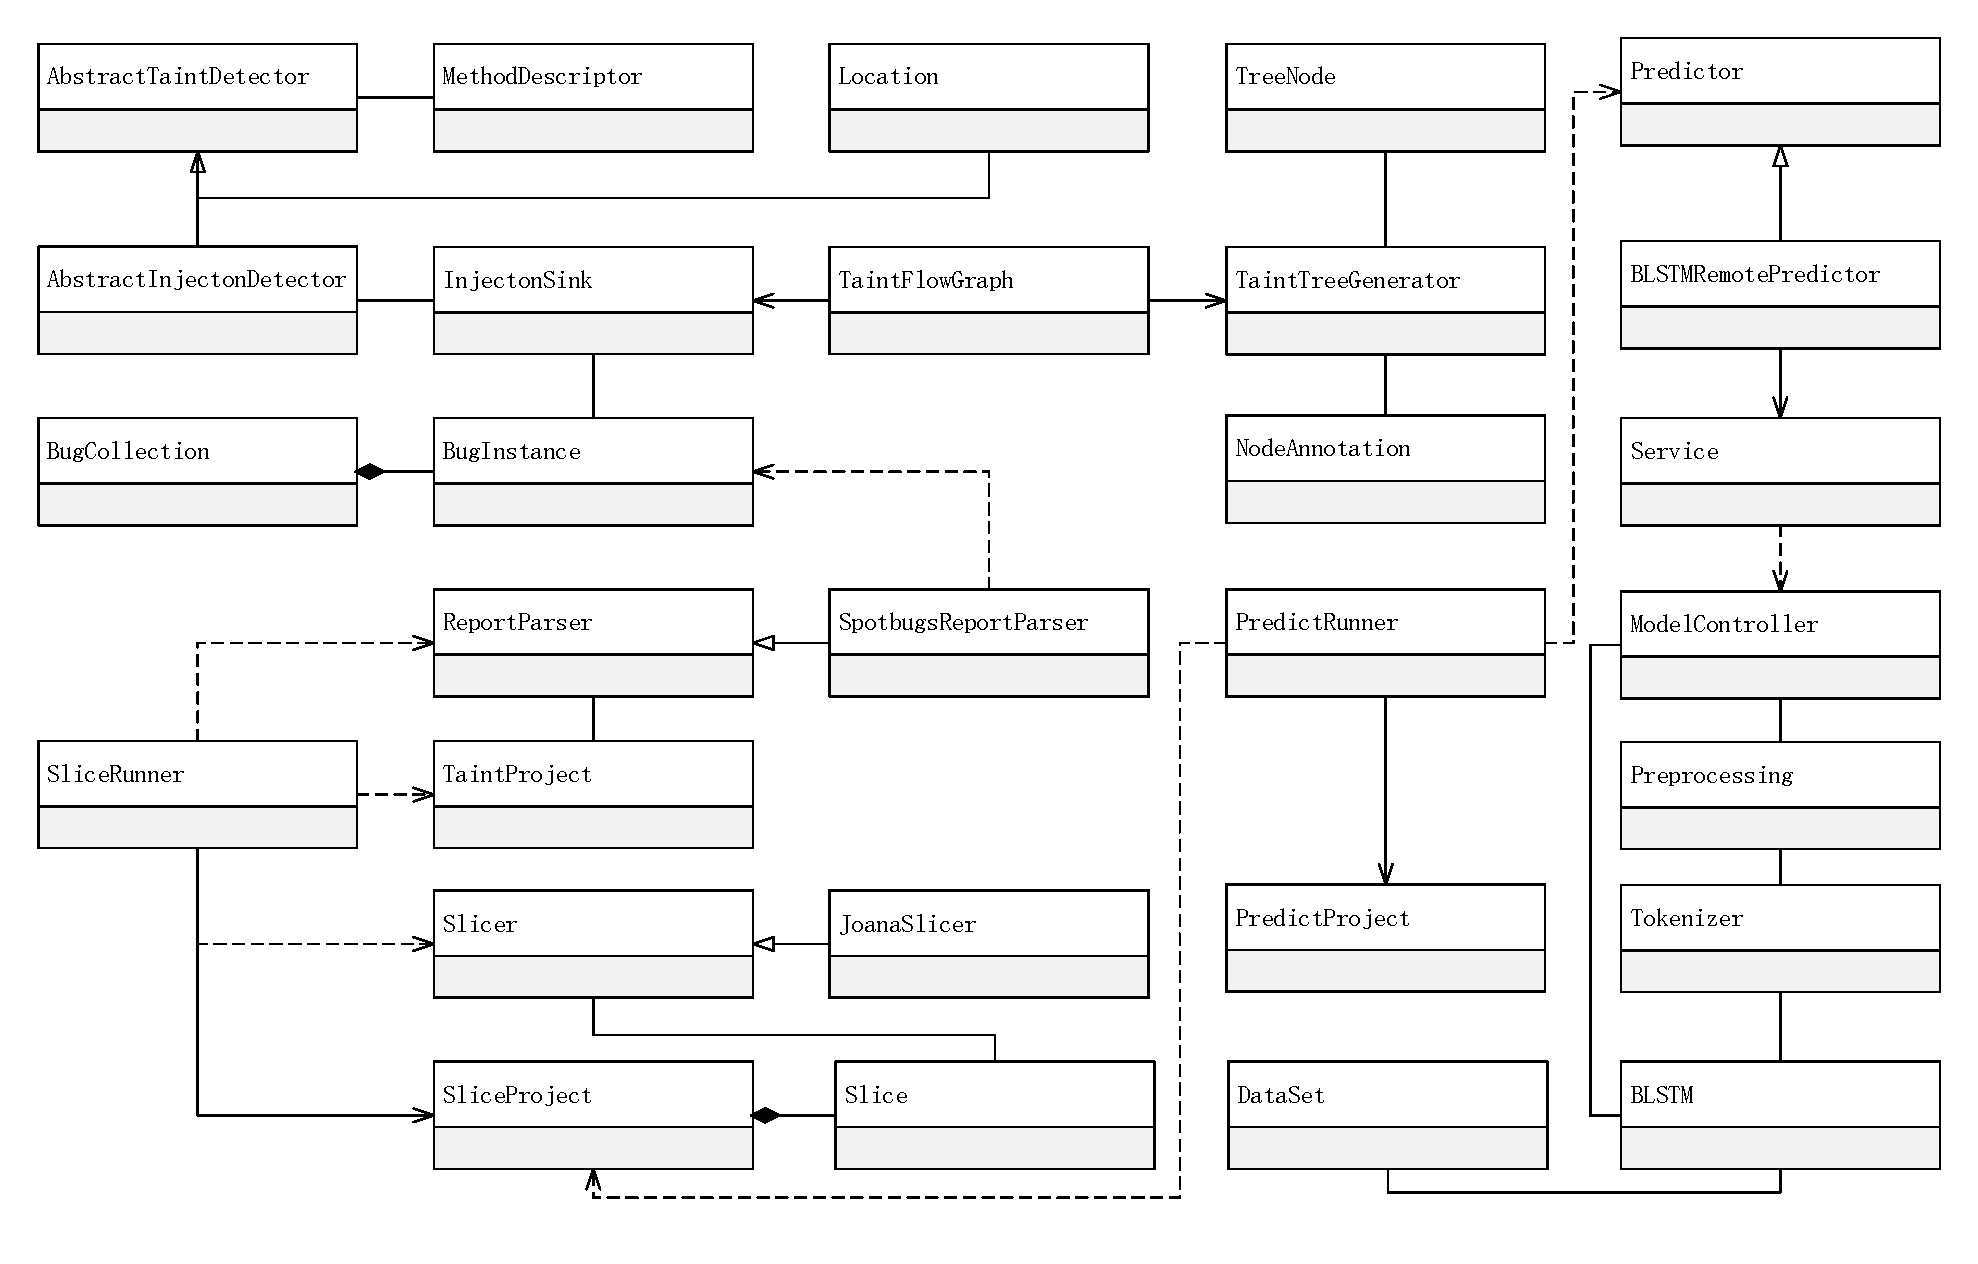
\includegraphics[width=5in]{FIGs/chapter3/viewlogic.pdf}
	\caption{系统逻辑视图}\label{view:logic}
\end{figure}

本系统的开发视图如图~\ref{view:dev}所示,该视图以开发者角度描述了模块的静态组织结构,具体来说本系统分为用户界面(UI),服务(Service)和第三方依赖包(Third-part Dependency)组成。

UI主要包括了客户端包和管理员Web端包;Service中存在污点分析(TaintAnalysis)包,切片(Slice)包,Joana切片器(Joana)包,预处理(Preprocessing)包,预测模块客户端包(PredictCli)和服务端(PredictSrv)包,以及用于表示各种数据的 Data 包;第三方依赖包中主要有 Spotbugs 和 FindSecBugs,Spotbugs 包含了基本GUI界面和数据流分析框架,FindSecBugs包括了基本污点分析引擎,Joana 为本系统选用的切片器,Pytorch 用于构建 BLSTM 模型,Django 框架用于构建后端服务,Celery 和 Redis 用于训练请求的异步调用。

\begin{figure}[!htb]
	\centering
	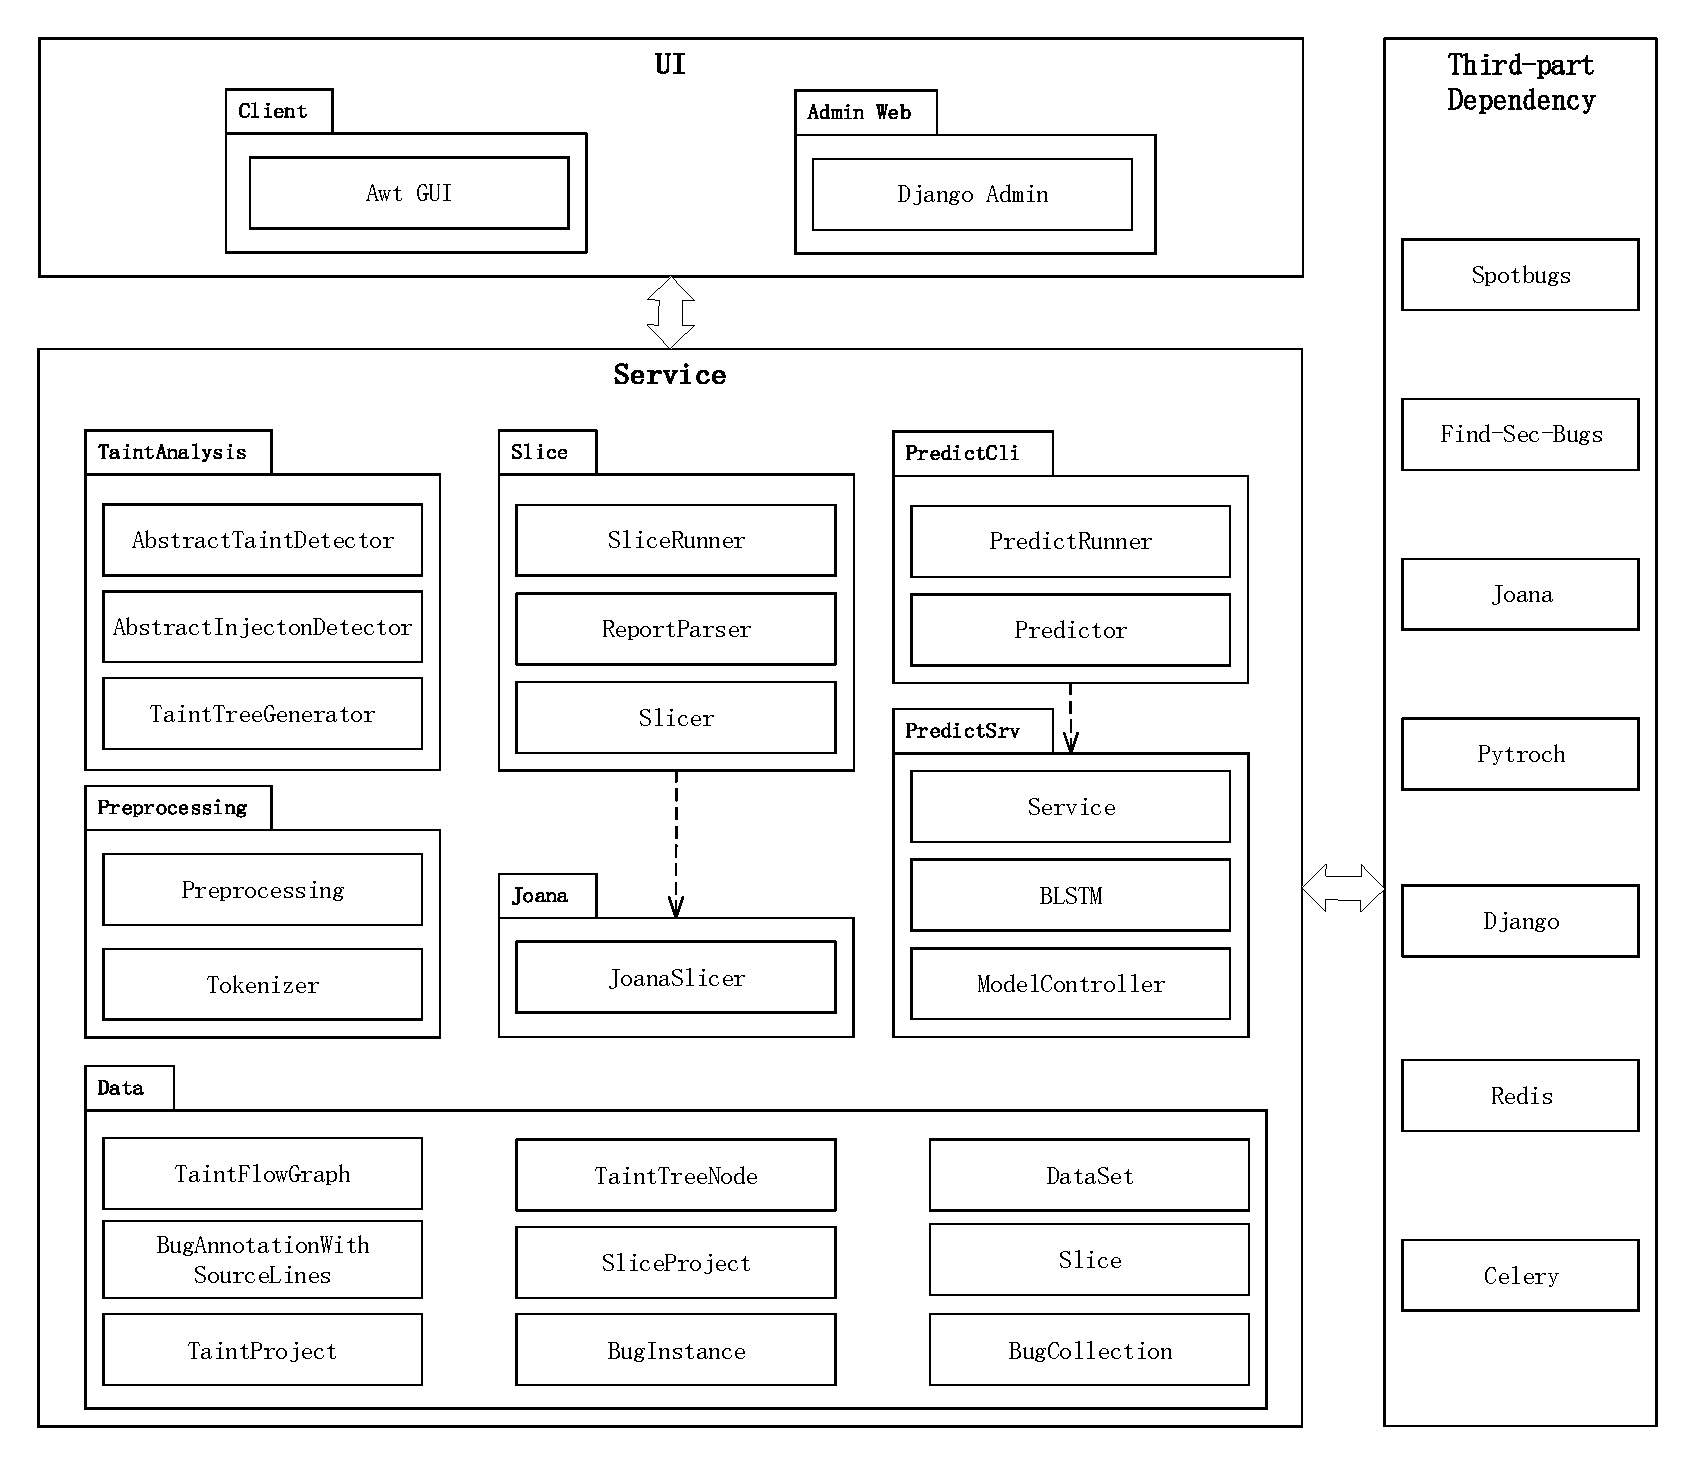
\includegraphics[width=5in]{FIGs/chapter3/viewdev.pdf}
	\caption{系统开发视图}\label{view:dev}
\end{figure}

本系统的进程视图如图~\ref{view:process}所示,用户端有管理端浏览器进程和代码扫描客户端进程,这两个进程通过 HTTP 协议与后端服务进程通信,服务进程通过TCP与模型训练任务进程和数据库进程通信,模型训练进程监听训练任务队列消息,收到训练消息后则开始模型训练,期间与数据库进程通信,获取训练配置信息。

\begin{figure}[!htb]
	\centering
	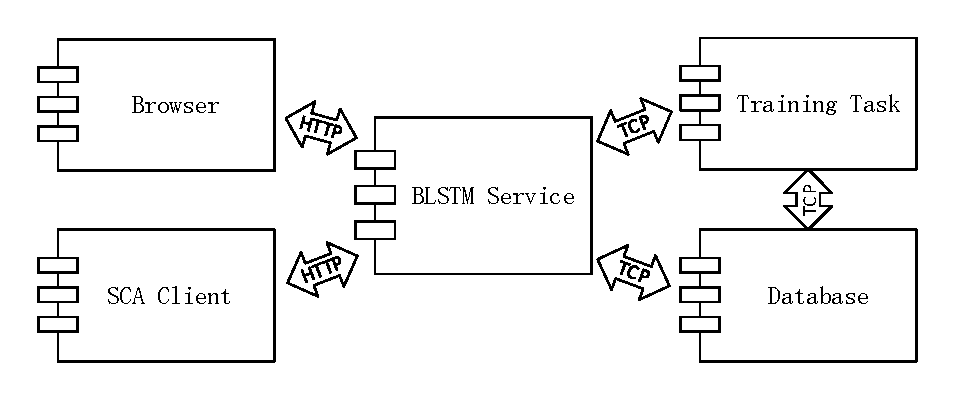
\includegraphics[width=0.7\textwidth]{FIGs/chapter3/viewprocess.pdf}
	\caption{系统进程视图}\label{view:process}
\end{figure}

本系统的物理视图如图~\ref{view:physical}所示,该视图在部署方面描述了本系统的架构。

在用户端部分,主要功能集中于扫描客户端,其包括了 GUI 界面和核心 jar 包(Core.jar),核心 Jar 包中含污点分析、切片和一部分预测模块。管理员用过浏览器使用本系统,主要完成发布模型训练任务、发放客户端 Token 或是管理数据对象的操作。

用户端通过HTTP与应用服务器通信,应用服务器上部署了基于BLSTM预测的 Web 应用,以及配置好的 Django 管理员后台应用,服务器上还部署了 Celery Work,以便使管理员可以发布关于模型训练的异步任务和定时任务,训练数据和已经训练好的模型直接存放在服务器的文件系统上。

服务端通过TCP与数据库连接,MySQL 数据库主要存放本系统的各种实体数据,Redis 数据库供 Celery 使用。
\begin{figure}[!htb]
	\centering
	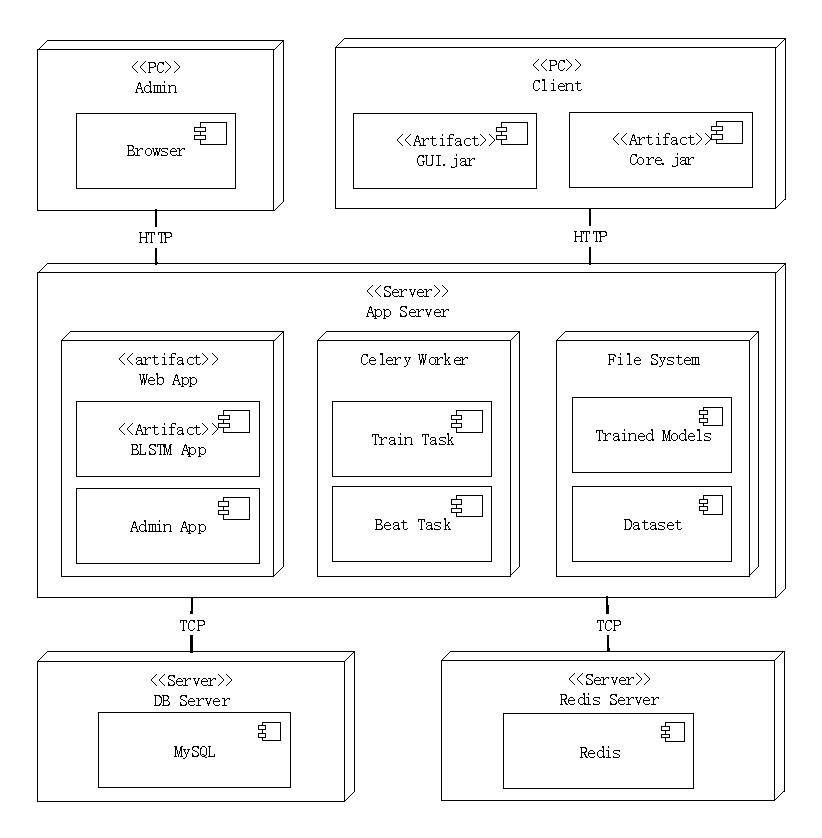
\includegraphics[width=0.7\textwidth]{FIGs/chapter3/viewphysical.pdf}
	\caption{系统物理视图}\label{view:physical}
\end{figure}

本系统的场景视图即用例图(图~\ref{fig:case}),在~\ref{sec:case} 章已经详细说明。

\section{污点分析模块设计}

污点分析模块是系统的基础模块,以用户提交的Jar包为输入,输出污点分析报告,本节分析流程和涉及到的类图两方面,说明该模块的设计。由于本模块主要是对FindSecBugs进行改进,使之可以在报告中输出污点传播树,因此本节只说明改进部分和与改进部分相关的类和流程,说明重点,对其它部分进行一部分简化。\\

\subsection{流程设计}
本系统的污点分析模块流程如图~\ref{taintprocess} 所示,首先用户输入被扫描的jar包对象,模块初始化漏洞报告,即产生一个空漏洞实例集合;接着其调用分析器对每一个类进行分析,对于第i个类,模块会对类函数的CFG进行拓扑排序,再依次对$i$类中的每个函数$k$进行污点分析,在污点分析时,本模块需要记录关于污点传播的有关信息,包括函数$k$内调用指令(如 \textit{invokestatic}、\textit{invokedynamic}、\textit{invokeinterface} 等)位置、函数返回指令位置(如 \textit{ireturn}、\textit{areturn}、\textit{dreturn} 等)和与污点汇聚点相关的代码语句位置信息,以便之后通过污点传播图和传播树产生漏洞报告。

污点传播最终报告内容为污点传播树,但是污点实际上是以图的形式进行传播的,因此本模块设计在漏洞报告阶段先生成污点传播图,再根据图生成污点传播树。

当应用中类和函数分析完后,模块会遍历所有污点汇聚点,这些污点汇聚点在分析时产生,记录了存在漏洞的汇聚点本身以及与污点传播到汇聚点的所有函数调用信息,对于每个汇聚点,利用汇聚点信息和分析时记录的函数调用语句位置,函数返回语句位置产生污点传播图。

最后,根据污点传播图构造污点传播树,并将传播树表示为能由GUI展示的漏洞实例对象,放入漏洞集合中,当所有汇聚点遍历完成后,模块最终输出漏洞实例的集合。

\begin{figure}[!htb]
	\centering
	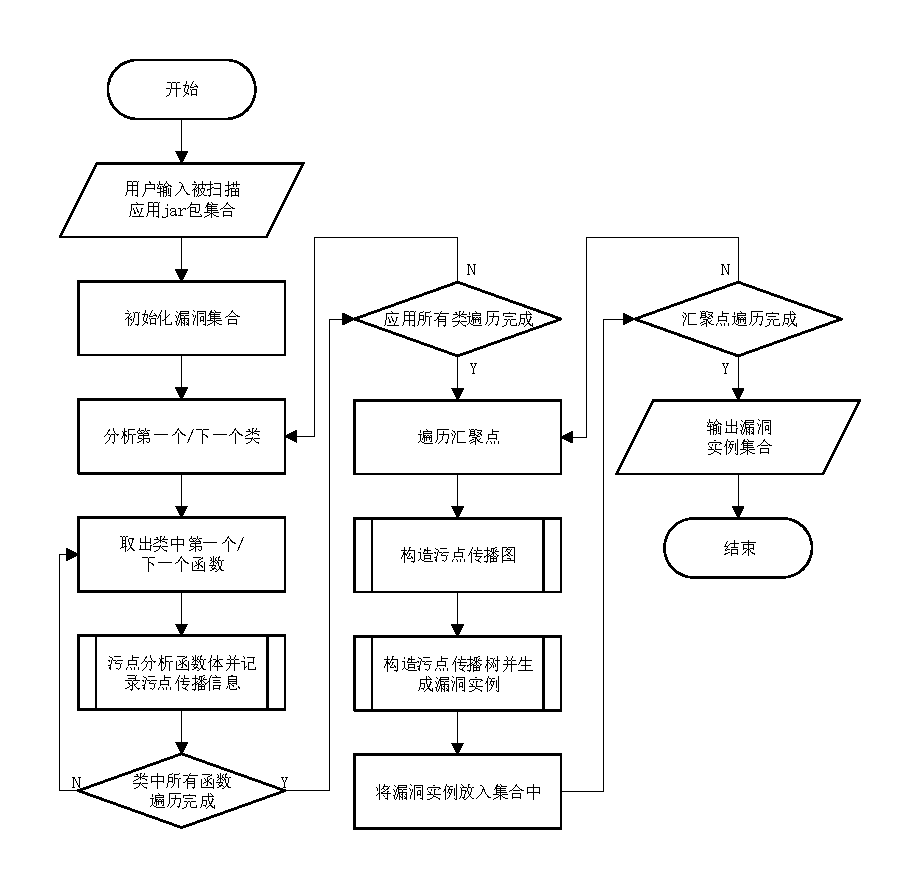
\includegraphics[width=0.8\textwidth]{FIGs/chapter3/taintprocessing.pdf}
	\caption{污点分析模块流程图}\label{taintprocess}
\end{figure}

图中记录污点传播信息、构造污点传播图和构造污点传播树的流程较为复杂,将在第~\ref{sec:taintImp} 节中详细说明。\\

\subsection{污点传播图类图设计}

为了方便图的遍历,污染传播图的数据结构采用邻接链表的形式,其类图设计如图~\ref{taintGraphClass} 所示。

\begin{figure}[!htb]
	\centering
	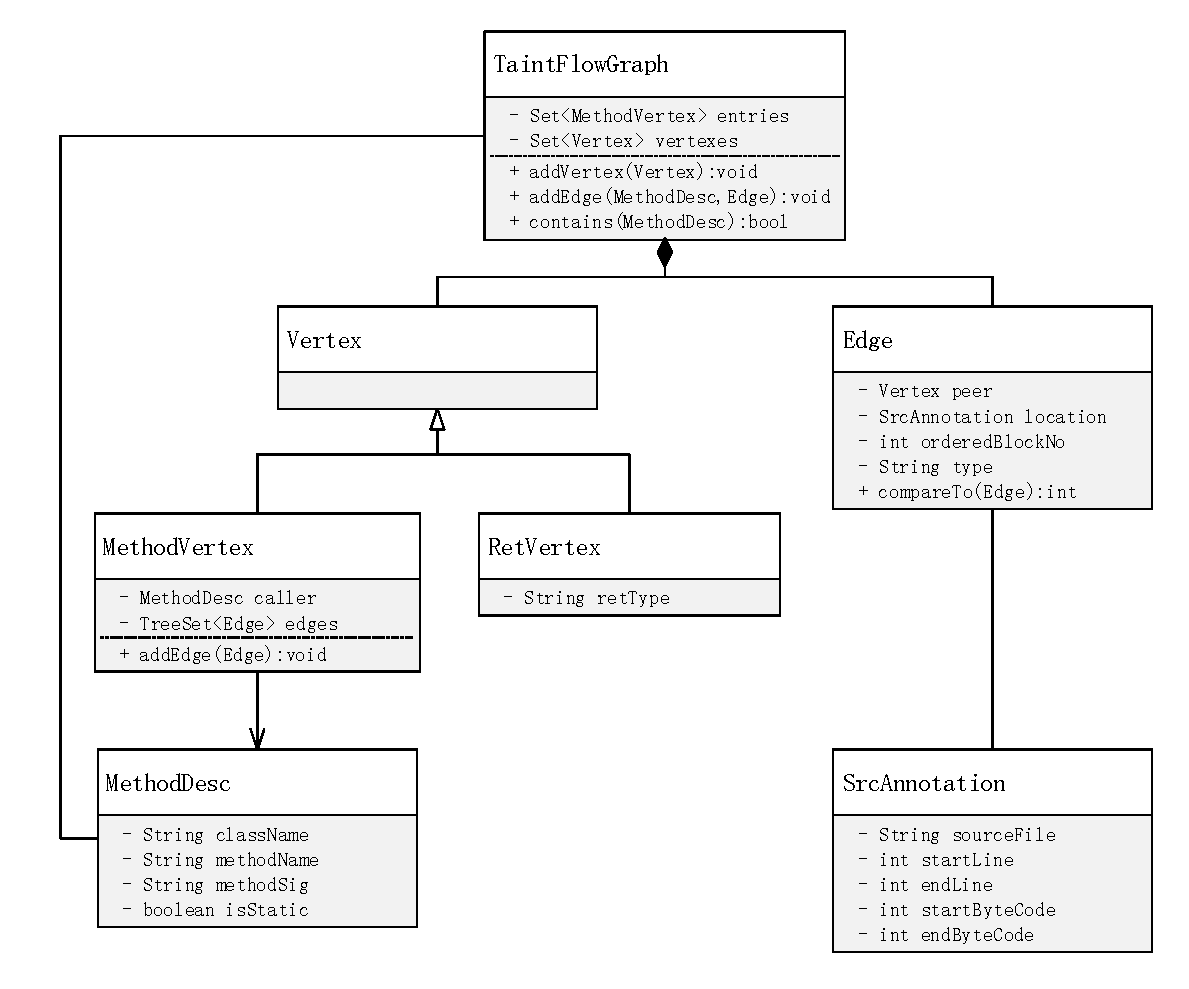
\includegraphics[width=0.8\textwidth]{FIGs/chapter3/taintGraphClass.pdf}
	\caption{污点传播图设计}\label{taintGraphClass}
\end{figure}

类 TaintFlowGraph 代表了一张污点传播图,图上的点由 Vertex 类表示,边由 Edge 类表示。TaintFlowGraph 中 entries 属性表示这张图入口函数的集合,这些函数只有出度没有入度,换句话说,污点在这些函数的上下文中传入,并传播至图中其他点,通常来说,这些函数有Web应用的视图层函数(如继承 \textit{HttpServlet} 子类中的 \textit{doGet()} 或 \textit{doPost()} 方法)或是客户端程序的入口函数(如 \textit{main()} 函数),该类中有向图中增加点的方法 \textit{addVertex()} 和向图中增加边的方法 \textit{addEdges()},还有一个检查函数摘要是否存在于图中的方法 \textit{contains()}。函数摘要类 MethodDesc 在系统逻辑视图中已出现过,该类主要用来唯一标识类中的函数,含有属性 className、methodName、methodSig 和 isStatic,分别表示类名,方法名,函数签名和是否为静态类。

顶点类 Vertex是一个抽象类,具体派生出表示函数的函数顶点类 MethodVertex 和 返回指令顶点类 RetVertex,MethodVertex 包含了一个函数摘要 caller ,以及该函数内连向其他顶点的边 edges,并且包含添加边的方法 \textit{addEdge()}。返回指令顶点类表示函数体中返回污点变量的返回值语句,其属性只有该语句类型 retType——通常来说 Java字节码 返回语句有 \textit{ireturn},\textit{dreturn},\textit{areturn} 等。不难发现,污点传播图上的顶点为函数或返回语句,并且只有 MethodVertex 才可以有出度,所以,在 TaintFlowGraph 类中的 \textit{addEdge()} 方法表示顶点的参数只能是一个函数摘要类型的顶点。

最后设计与边相关的类,Edge 类,该类表示这一条边和连接这一边的对端顶点,peer 属性表示对端顶点, location 代表了两点之间通过哪一个代码位置与之相连,type 指这条边的类型,模块中主要有三种类型(“CALL”,代表函数调用;“SINK”,代表调用到汇聚点,“RET”,代表函数返回),blockId 属性表示这条边所在的代码块,该属性的目的是为了结合 CFG 将污点传播图拆解为传播树,以及保证边的顺序。代码位置有SrcAnnotation 该类将在下一章详细说明。\\

% 是否要举个例子或者话一张该图的数据结构?

\subsection{污点传播树和漏洞报告类图设计}

污点传播树是展示污点传播过程的重要数据结构,其中叶子结点中有一污点入口点和一污点汇聚点,其他叶子节点为函数或返回语句节点,树的层级关系反映出函数调用关系,一棵传播树代表了一个唯一的污点传播全流程,其结构体和漏洞报告类图设计如图~\ref{taintTreeAnnotationClass}所示。

对于污点传播树,有一工具类TaintTreeGenerator,主要有两个方法:\textit{makeTree()} 和 \textit{makeAnnotation()},\textit{makeTree()} 方法输入为污点传播图的一个入口点,根据这一入口点构造若干棵传播树;\textit{makeAnnotation()}根据污点传播树构造出一注解列表,这些注解列表最终在GUI界面上展现污点传播树。

考虑到污点传播树存在树形结构,并且节点存在运行顺序的上下关系的特征,本模块设计使用树的孩子兄弟结构来表示污点传播树。TreeNode 表示树上节点对象,其 id 表示了该节点的序号,其主要用来在反序列化时重构树;location 属性表明了该节点在程序中的位置,type 表示节点类型,在本系统中,该类型种类和传播图的 Edge 类型一致;firstChild 为 TreeNode 对象,指向其第一个子节点,具体来说,父节点是一个函数节点,而子节点可以使函数节点或是返回节点;nextSib 为 TreeNode 对象,指向同一深度的下一个叶子对象,具体地说,是同一函数上下文下的下一对象。TreeNode 派生出两类节点,一个是表示函数的节点 MethodTreeNode,其有一类型为 MethodDesc 的属性 caller,另一个是表示返回语句的节点 RetTreeNode,其有一属性 retType 表示了返回语句类型,与上文 RetVertex 类型一致。

% 是否要举个例子或者画一张该图的说明该注解还以?
漏洞注解类 BugAnnotation 、漏洞实例 BugInstance 类和漏洞实例 BugCollection 类都是 Spotbugs 定义的数据类型,漏洞注解类该类表示了对漏洞的一行解释性文字。
BugInstance 是应用中一个漏洞的基本单位,其有一个漏洞类型(type 属性)和多行漏洞注解(list 属性)组成。在 BugAnnotation 中, \textit{format()} 是该条注解在GUI界面上的显示文字时被调用的方法,\textit{writeXML()} 用于将注解保存为XML格式,以上为原生 Spotbugs 定义的方法,除此之外,为了方便反序列化,本模块还为其增加了 \textit{fromXML()}方法。NoteAnnotation、RetNodeAnnotation 和 MethodNodeAnnotation 对应于污点传播树的 TreeNode、RetTreeNode 和 MethodTreeNode 节点,对于抽象的节点注解类 NoteAnnotation 而言,其id、firstId,nextId 分别指向了 TreeNode的id,第一个孩子节点的id和第一个兄弟节点的id,depth 表示该节点距离树根的深度,具体类 RetNodeAnnotation 和 MethodNodeAnnotation 会将重现实现 BugAnnotation 类的三个方法,特别的,RetNodeAnnotation 的 firstId 恒为-1,因为返回语句的节点不会存在子节点。BugCollection类主要有漏洞实例组成,除此之外,其还记录有项目名称,用户提交的应用jar包(appJars)、依赖包(libJars)和源码包(srcs)。


\begin{figure}[!htb]
	\centering
	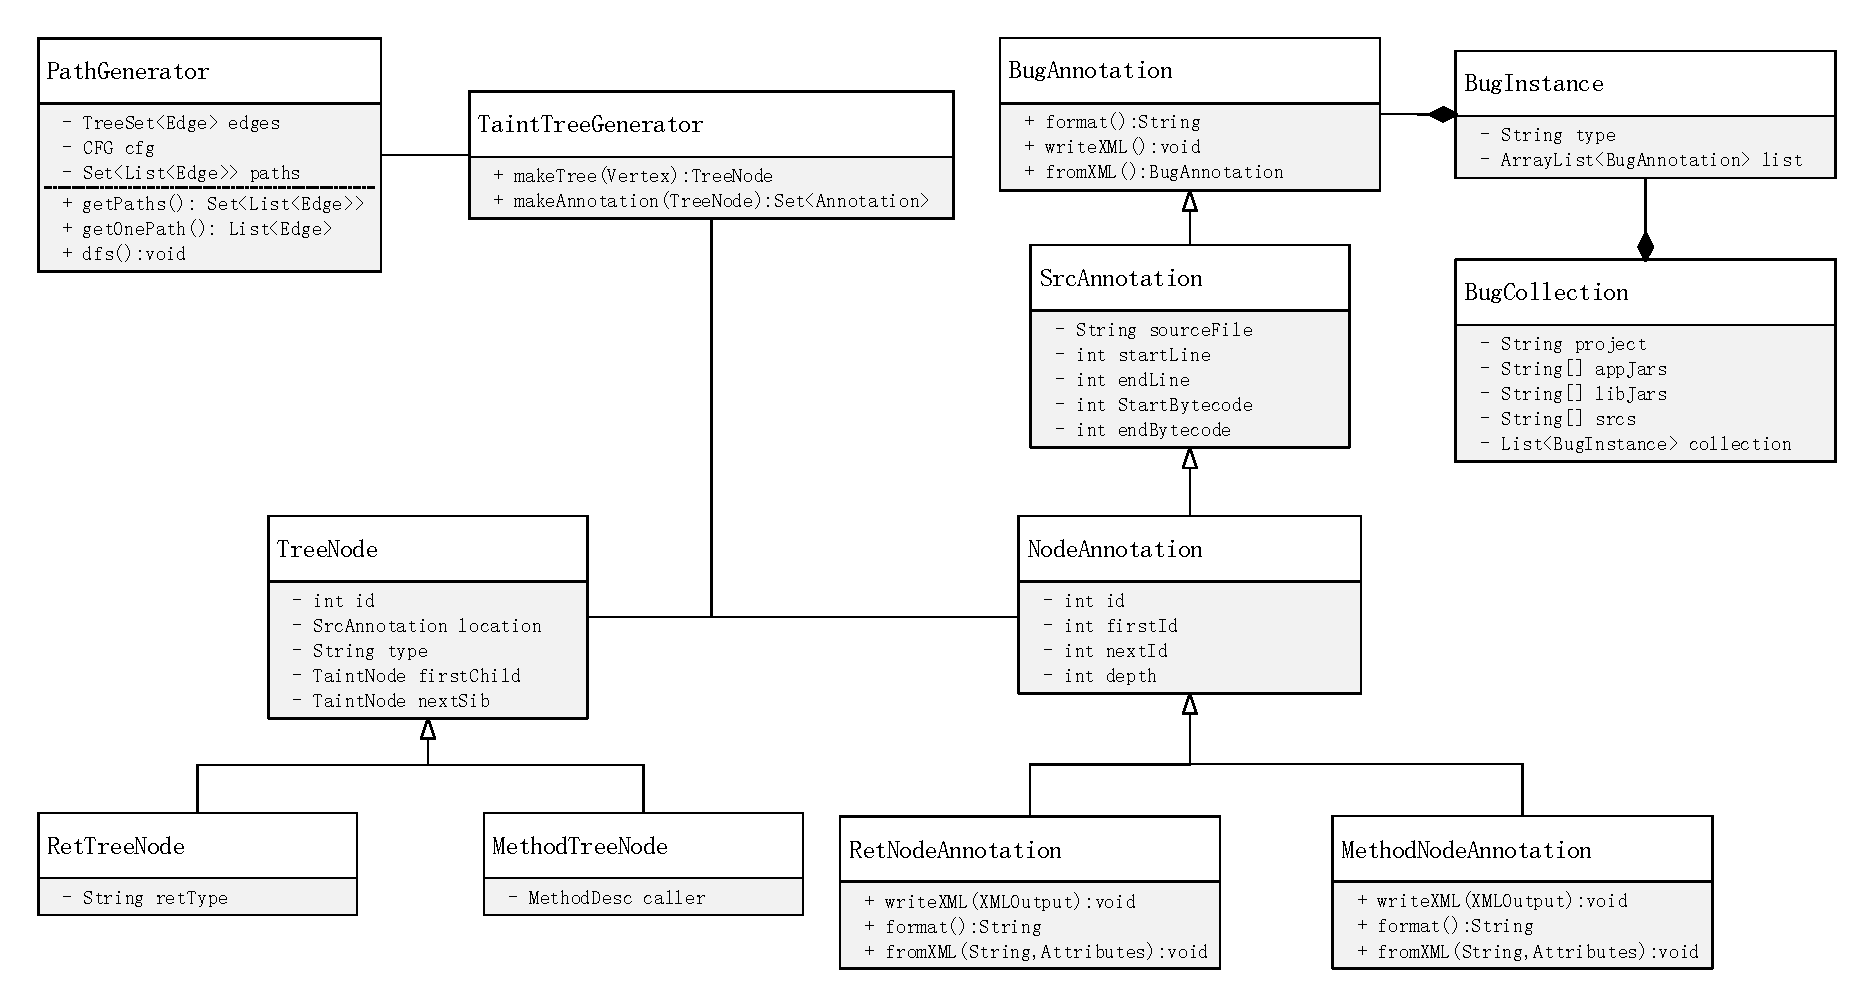
\includegraphics[width=0.8\textwidth]{FIGs/chapter3/taintTreeAnnotationClass.pdf}
	\caption{污点传播树和漏洞报告类图设计}\label{taintTreeAnnotationClass}
\end{figure}

\subsection{污点分析器类图设计}

污点分析器类图设计如图~\ref{taintDetectorClass}所示,Detector 类是所有分析器的基类,对于每一个 Detector 子类,Spotbugs会按流程图~\ref{taintprocess}所示使其分析目标 Jar 中的每个类,其中调用的就是类中 \textit{visitClassContext()} 方法,类遍历完成后,又会调用 \textit{report()} 方法产生报告。
\begin{figure}[!htb]
	\centering
	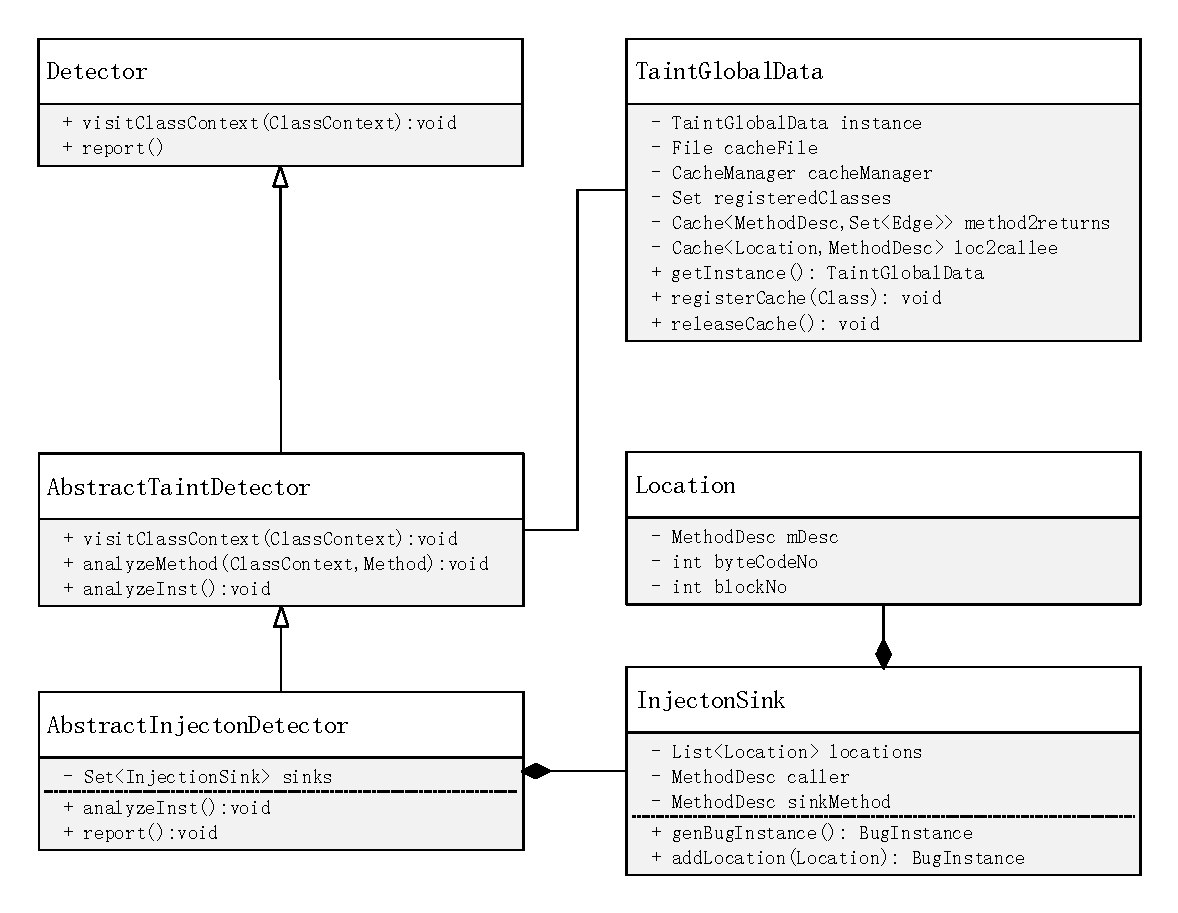
\includegraphics[width=0.8\textwidth]{FIGs/chapter3/taintDetectorClass.pdf}
	\caption{污点分析器类图设计}\label{taintDetectorClass}
\end{figure}

AbstractTaintDetector 继承 Detector 类,该类也是记录污点传播信息的重要基类,其关键在于 returns 属性和 loc2callee 属性,returns记录了每一个函数中能够返回污点变量的 return 语句,loc2callee 记录了在函数调用发生时,invoke指令所在的函数位置和被调用的函数摘要。其会实现 Detector 的 \textit{visitClassContext()} 方法,并且在该方法内,调用 \textit{analyzeMethod()} 方法对每一个目标函数进行分析,对于污点传播信息的记录逻辑也在该方法内。对于特殊指令,如 \textit{return} 和 \textit{invoke},\textit{analyzeMethod()} 会调用  \textit{analyzeInst()} 对指令进行分析。

AbstractInjectionDetector 继承了 AbstractInjectionDetector,进一步实现了污点分析过程,即实现了 \textit{analyzeInst()} 和 \textit{report()} 方法,其属性 sinks 记录了目标应用的所有汇聚点,在所有类的分析完成后,依次调用 \textit{report()} 生成报告。

污点汇聚点的类名为 InjectionSink,其属性 caller 和 sinkMethod 为调用敏感函数的最后一个函数,以及敏感函数的函数摘要,除此之外,所有将污点汇聚到该点的调用语句有被记录在其 locations 列表上,\textit{addLocation()} 就是记录调用语句发生位置的方法,\textit{getBugInstance()} 方法为产生报告的具体方法,被 \textit{AbstractInjectionDetector.report()} 方法调用,构造污点传播图、传播树和生成漏洞实例逻辑都在该方法中。

上面提到的位置信息由 Location 类表示,其包含的属性有语句所在函数的函数摘要(mDesc),语句所在的字节码序号(byteCodeNo)和所在 CFG 代码块的序号(orderedBlockNo)。



\section{程序切片模块设计}

程序切片模块是误报预测的基础,本系统优化了前人工作,能够对一个漏洞进行完整切片,本节从流程设计类图设计两方面介绍该模块的设计。\\
\subsection{流程设计}

本模块的流程设计如图~\ref{sliceProcessing} 所示,该模块的输入是用户提交的项目 Jar 包和在上一模块已经产生的漏洞报告中的漏洞实例集合,其输出是切片项目类,从类图分析可知,该项目类中含有所有漏洞及对应的所有切片。

\begin{figure}[!htb]
    \centering
    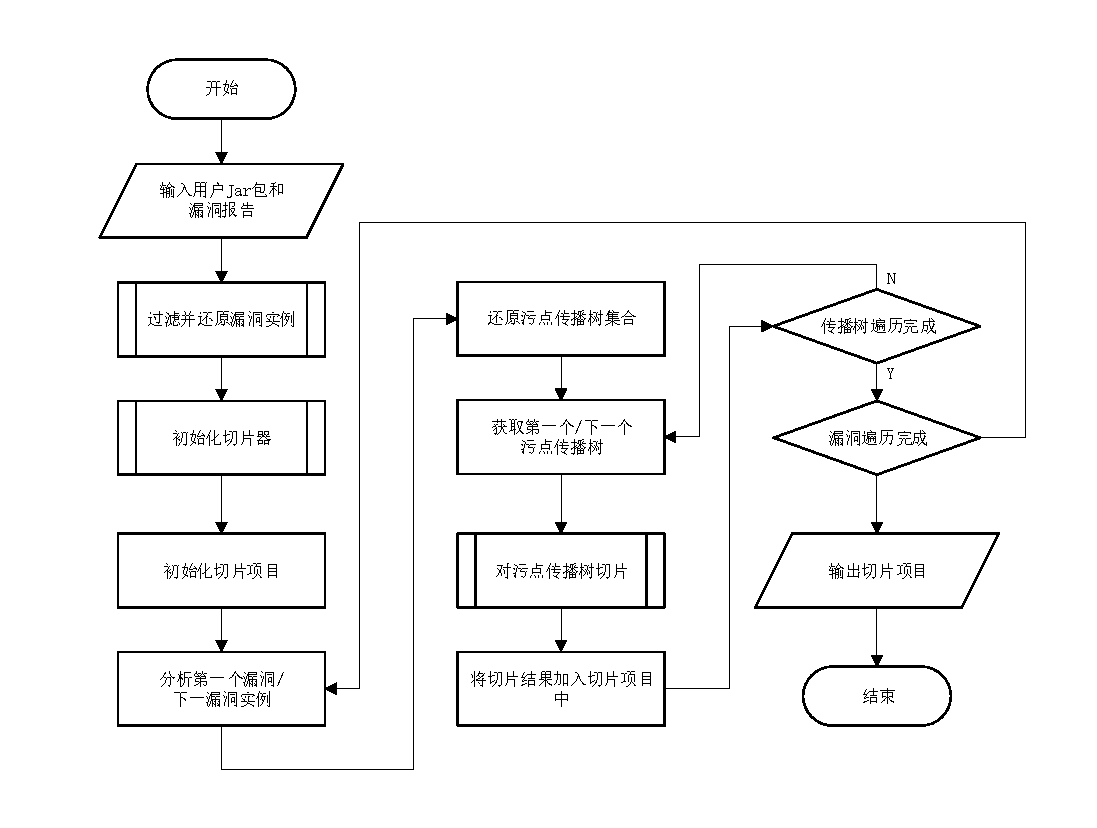
\includegraphics[width=0.8\textwidth]{FIGs/chapter3/sliceProcessing.pdf}
    \caption{程序切片模块流程图}\label{sliceProcessing}
\end{figure}

因为 Spotbugs 中除了上文提到的污点传播检测器还存在其他漏洞检测器,其他检测器产生漏洞不属于本系统处理范围,在模块运行前,先要对漏洞报告进行过滤,同时将污点传播类型的漏洞反序列化漏洞注解,接着模块初始化一个具体的程序切片器,其中包括了对切片器的各种配置,具体会在实现章节介绍,以及初始化一个空的切片项目。接下来将会遍历漏洞实例集合中的每一个漏洞,对于一个污点传播漏洞,根据上一模块产生的漏洞实例注解集,还原出若干棵污点传播树,接下来就是对污点传播树进行拆解并切片的步骤,该步骤是本系统的核心步骤之一,包括了对污点传播树进行拆解,将其分为污点传播流作为为更小的切片任务,其具体实现也将在下一实现章节介绍;对污点传播树的切片结束后,将传播树信息和对应切片集合加入项目中,遍历完所有漏洞的污点传播树后,模块输出切片项目,项目内存在与漏洞相关的所有切片。\\

\subsection{类图设计}

\begin{figure}[!htb]
    \centering
    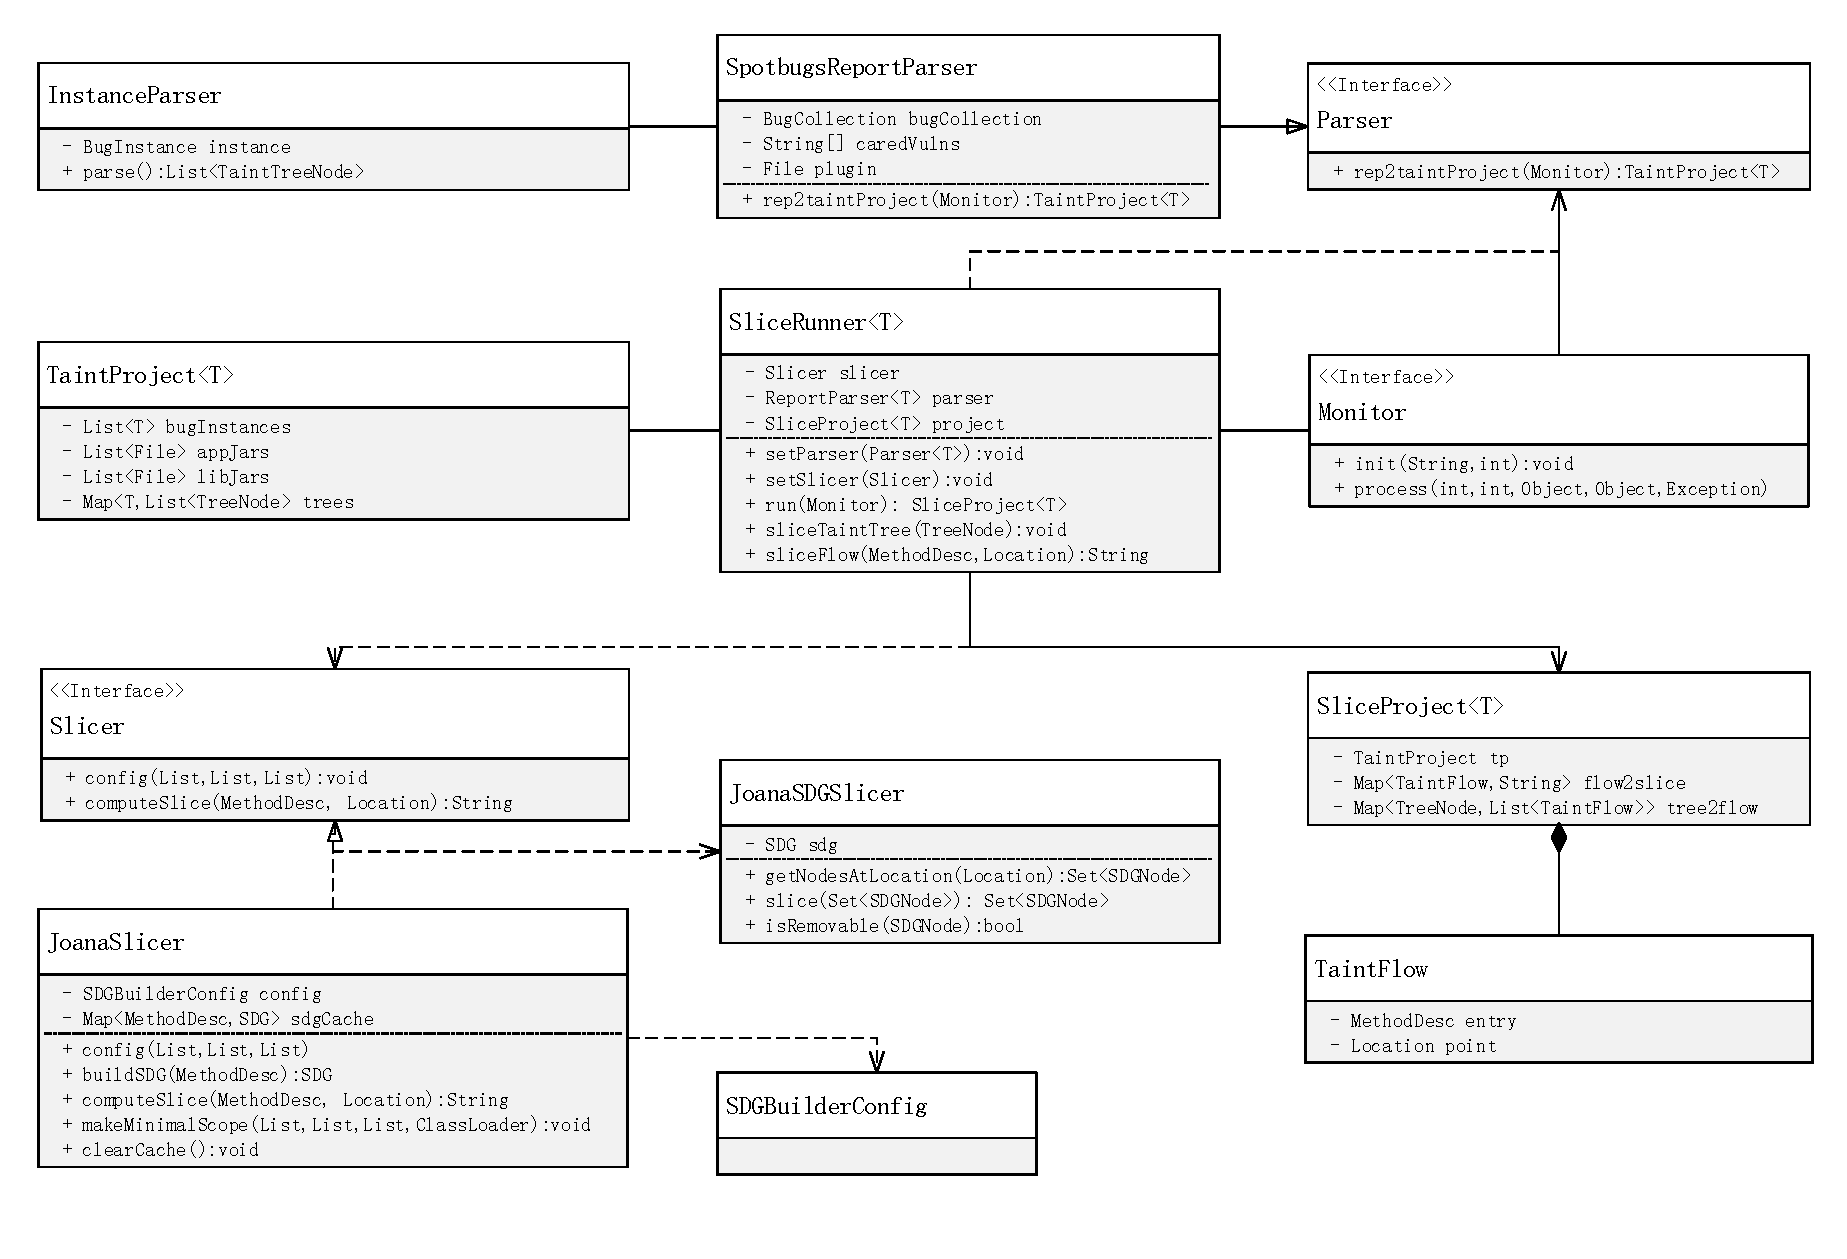
\includegraphics[width=0.9\textwidth]{FIGs/chapter3/sliceClass.pdf}
    \caption{程序切片模块类图}\label{sliceClass}
\end{figure}

本模块的类图设计如图~\ref{sliceClass} 所示。首先介绍模块的核心控制类 SliceRunner,该类用于读取污点传播报告,并最终产生每一漏洞实例的切片集合,其有三个属性成员:slicer,表示用于切片的切片器;parser,污点传播报告的翻译器;project,最终输出的切片项目。切片器和翻译器分别由 \textit{setSlicer()} 和 \textit{setParser()} 设置,\textit{run()} 方法是对漏洞报告切片的控制方法,其参数是一个监视器,上一章节所说的模块流程将在该方法内完成,\textit{sliceTaintTree()} 是对一个污点传播树切片的方法,可以看到其参数是一个树节点表示该传播树的树根,\textit{sliceFlow()} 是对一个传播流切片的方法。

Monitor 类是监视器接口,用于方便各种耗时较长的函数中间返回信息,具体地说,该接口的 \textit{init()} 方法用于通知类开始某一流程,第一个参数为过程名,第二个参数表示过程共几个子过程;\textit{process()} 方法用于在每一个子过程完成后调用,其参数依次向监视器发送了当前子过程序号,过程总数,子过程输入,子过程输出,以及遇到的异常。该接口规范了系统内的任务进度报告模式,使外部能够自由的处理每一子过程并及时通知用户(例如,在每一子过程完成时向屏幕输出进度或是处理异常),除了切片控制类会使用该类外,未来的预测控制类也会使用。

接下来设计与污点传播翻译器相关的类,Parser 是翻译器接口,其 \textit{rep2taintProject()} 方法用来将漏洞报告翻译为一个污点传播项目,同样,其也有一个监视器作为参数。 SpotbugReportParser 实现了该接口,其属性有 bugCollection,该属性在类初始化时传入,表示污点传播报告,caredVulns 表示污点传播漏洞类型白名单,该属性为静态属性,plugin 为本系统优化后的 FindSecBugs 插件(注意到反序列化函数 \textit{fromXML()} 在插件中)。SpotbugReportParser 的 parse() 方法将漏洞报告转化为了污点传播项目,而真正将漏洞实例还原为若干棵污点传播树的是来自 InstanceParser 类中的 \textit{parse()} 方法,该类成员变量 instance 为一漏洞实例,在类构造时传入。翻译的最终产出是 TaintProject 对象实例,该类中 bugInstances 表示了所有的污点传播方法,appJars 和 libJars 表示了用户提交的应用 Jar 包集合和第三方依赖 Jar 包集合,trees 为一组键值对,记录了一个 bugInstance 的所有污点传播树的树根节点。

Slicer 是切片器的接口,\textit{config()} 方法用来配置一个切片器,其中三个列表参数分别代表引用 Jar 包,第三方依赖 Jar 包和黑名单类,当切片内容在黑名单类的上下文时,该条切片被舍弃,这主要用来过滤 Java Runtime 中的切片,或者排除其他第三方包的切片。\textit{computeSlice()} 方法是对一个污点传播流的切片方法,其参数是指以 MethodDesc 的函数为入口进行对关注点 Location 的切片,切片返回String类型,每条切片用“$\backslash$n”分割。 JoanaSlider 类是 Slicer 的一个具体实现,其 config 变量表示一个用于保存生成SDG 的配置信息,配置类名为 SDGBuilderConfig,由于该类涉及到实现细节,将在下一章进行讨论, sdgCache 用于缓存SDG,类中除了实现 \textit{config()} 和 \textit{computeSlice()} 方法,还有构造 SDG 的方法 buildSDG(),其参数为 SDG 的入口函数的函数摘要,\textit{makeMinimalScope()} 方法为构造最小搜索范围方法,被构造 SDG 时使用,clearCache() 方法用于清除各类缓存,在构造 SDG 后,主要切片工作由 JoanaSDGSlicer 梳理,该类在创建时传入 SDG 作为属性,先通过 \textit{getNodesAtLocation()} 获取关注点的 SDGNode,再通过 \textit{slice()} 方法切出所有相关的 SDGNode,并且通过 \textit{isRemovable()} 函数将一些无效节点删除(如非函数语句节点,抽象类节点等)。

切片模块最终返回切片项目类 SliceProject 对象,该对象内部持有一污点传播项目对象,从传播树到污点传播流的映射(tree2flow 属性)和从污点传播边到切片的映射(edge2slice 属性)。TaintFlow 对象代表污点传播流,可以看到,其属性 entry 和 point 正好对应了切片器接口切片函数的参数,它的实际上代表了污点在一个函数内传播的过程。

从本模块的类图设计上可以看出,本模块基本上实现了对切片器和污点分析器的解耦,在某些类上的泛型 T 表示了漏洞类型类,考虑到了今后不同污点分析工具的返回漏洞类型不同这一情况,即使今后需要换用其他污点分析引擎或是切片器,只需要重新实现 Parser 和 Slicer 再修改泛型就可重用本模块。

\section{数据预处理模块设计}

数据预处理模块是预测过程中承上启下的模块,其接受切片数据,并将其泛化和向量化,使之可以输入 BLSTM 模型。本节从模块流程类图设计和流程设计两方面介绍模块的设计思路。\\


\subsection{流程设计}

\begin{figure}[!htb]
    \centering
    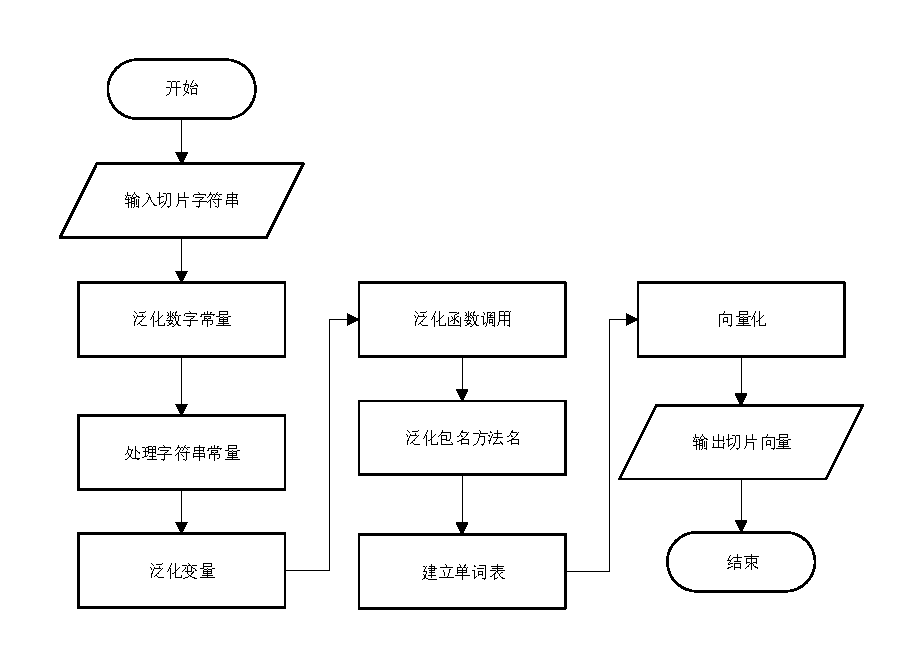
\includegraphics[width=0.9\textwidth]{FIGs/chapter3/preProcessing.pdf}
    \caption{数据预处理模块类图}\label{preProcessing}
\end{figure}

图~\ref{preProcessing} 展示了本模块的流程图,首先模块输入上一模块产生的切片字符串,接着字符串经过各类泛化处理,变为由空格分隔单词字符串,再根据该字符串构建单词表(注意,在构建的单词表会对低频词过滤,其本质仍为泛化处理),最后通过查表完成字符串的向量化,最终模块输出切片向量。

泛化处理是模型准确性的重要保障,针对本系统应用场景,模块依次完成了五类泛化处理,即泛化数字常量,泛化字符串常量,泛化变量,泛化函数调用和泛化包名及方法名,其具体做法将在实现章节说明。\\

\subsection{类图设计}

\begin{figure}[!htb]
    \centering
    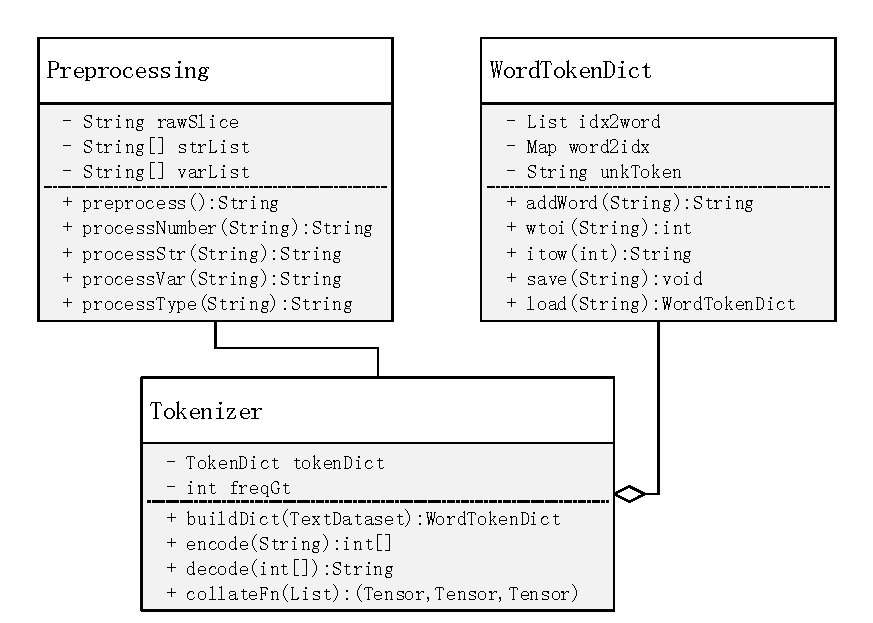
\includegraphics[width=0.9\textwidth]{FIGs/chapter3/preClass.pdf}
    \caption{数据预处理模块类图}\label{preClass}
\end{figure}

图~\ref{preClass} 展示了本模块的类图,Preprocessing 类用于对切片数据进行泛化理,其 rawSlice 属性为原切片字符串,strList 为字符串常量表,varList 为变量常量表,其 \textit{preprocess()} 方法为主要的泛化方法,输出以空格分隔的单词(token)。\textit{processNumber()} 、 \textit{processStr()} 和 \textit{processVar()} 分别是泛化数字常量、字符串常量和变量的方法,它们的输入为一行切片,输出为泛化后的切片字符串。processType() 为泛化返回值类型的方法,其输入为一返回值类型字符串,输出为泛化后字符串。

Tokenizer 类用于将泛化后字符串转换为一维向量(向量化),其属性 freqGt 值只有当单词在数据集中出现频率大于改值时单词才有效,其还包含一单词表对象 tokenDict,\textit{buildDict()} 用于构造一个单词表,其输入为 pytorch 中定义的TextDataset,通过该对象可以遍历数据集中每一条数据,其输出为单词表。\textit{encode()} 方法用于将泛化字符串边为向量,\textit{decode()} 是其反函数,用于将向量还原成字符串。

TokenDict 为单词表类,用于记录单词和其整形 id 的对应关系,其属性 idx2word 和word2idx 分别记录了 id 至单词,和单词至 id 的对照表,属性 unkToken 记录了未知单词的值(默认为“$\langle UNK \rangle$ ”),\textit{addWord()} 方法是实现了将一单词放入单词表中,\textit{wtoi()} 和 \textit{itow()} 是一对互逆操作,用于将单词转换为数字 id,以及将 id 还原为单词, \textit{save()} 和 \textit{load()} 分别实现了将单词表保存为文件,以及从文件中反序列化为单词表的操作。

\section{误报预测模块设计}

预测模块是系统最后也是最重要的模块之一,该模块参考先前研究者的工作,通过机器学习的预测漏洞是否为误报,从而提高扫描结果的准确性。本节将通过架构设计、类图设计、流程设计三个方面介绍该模块的设计。\\

\subsection{架构设计}

相较于先前模块,预测模块的特殊之处在于其不只存在于一处硬件资源上(其跨越了客户端和服务器),由于其结构较为复杂,因此本节首先介绍模块的架构设计,其架构图如图~\ref{predictArch}所示。

\begin{figure}[!htbp]
    \centering
    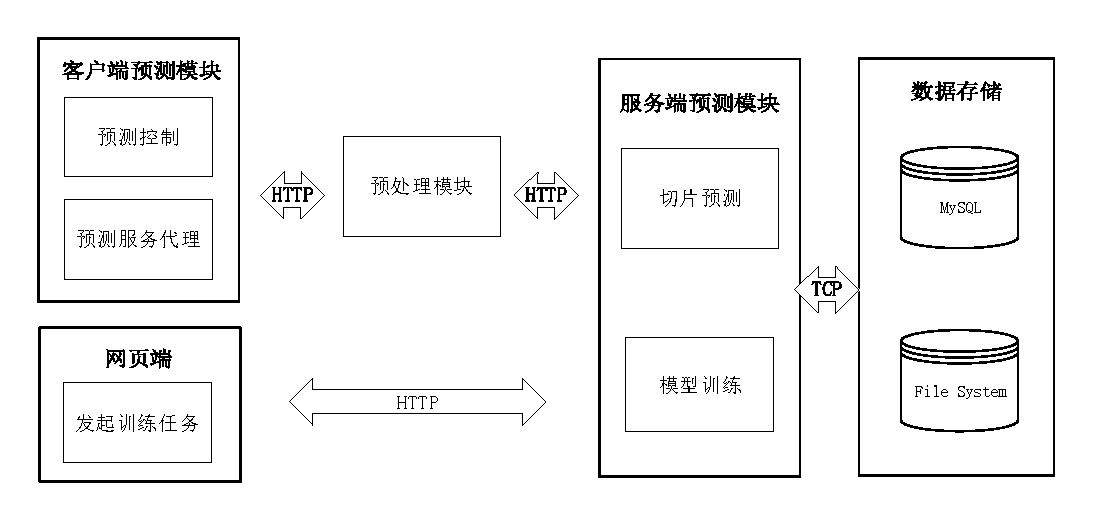
\includegraphics[width=0.8\linewidth]{FIGs/chapter3/predict-architecture.pdf}
    \caption{预测模块架构图}\label{predictArch}
\end{figure}

预测模块的一部分存在于客户端中,其作用在于代理远程服务器,以及对于一个漏洞实例中的每一个传播树中的每一个传播流切片进行预测,再根据预测结果判断一个实例是否是误报——预测控制。预测服务代理会将原始切片内容发送给预处理模块,预处理模块转化后将向量发送给服务端。

服务端预测模块主要功能有基于 BLSTM 模型,对于单个污染流切片进行预测、切片标记以及将标记数据和切片存储于数据库和本地系统中。同时用户可以直接通过网页端,发起训练任务,模型训练任务同样也在服务端预测模块中完成。\\

\subsection{类图设计}

本模块类图如图~\ref{predictClass} 所示,在客户端,有预测控制类 PredictRunner、预测器类 Predictor、切片类 Slice、标记类 Label、远程预测器代理类 BLSTMRemotePredictor、预测项目类 PredictProject 和预测器异常类 PredictorException;在服务端,有预测服务类 Views,模型控制类 ModelController,模型效果度量类 MetricCalculator 和神经网络模型类 BLSTM。

\begin{figure}[!htbp]
    \centering
    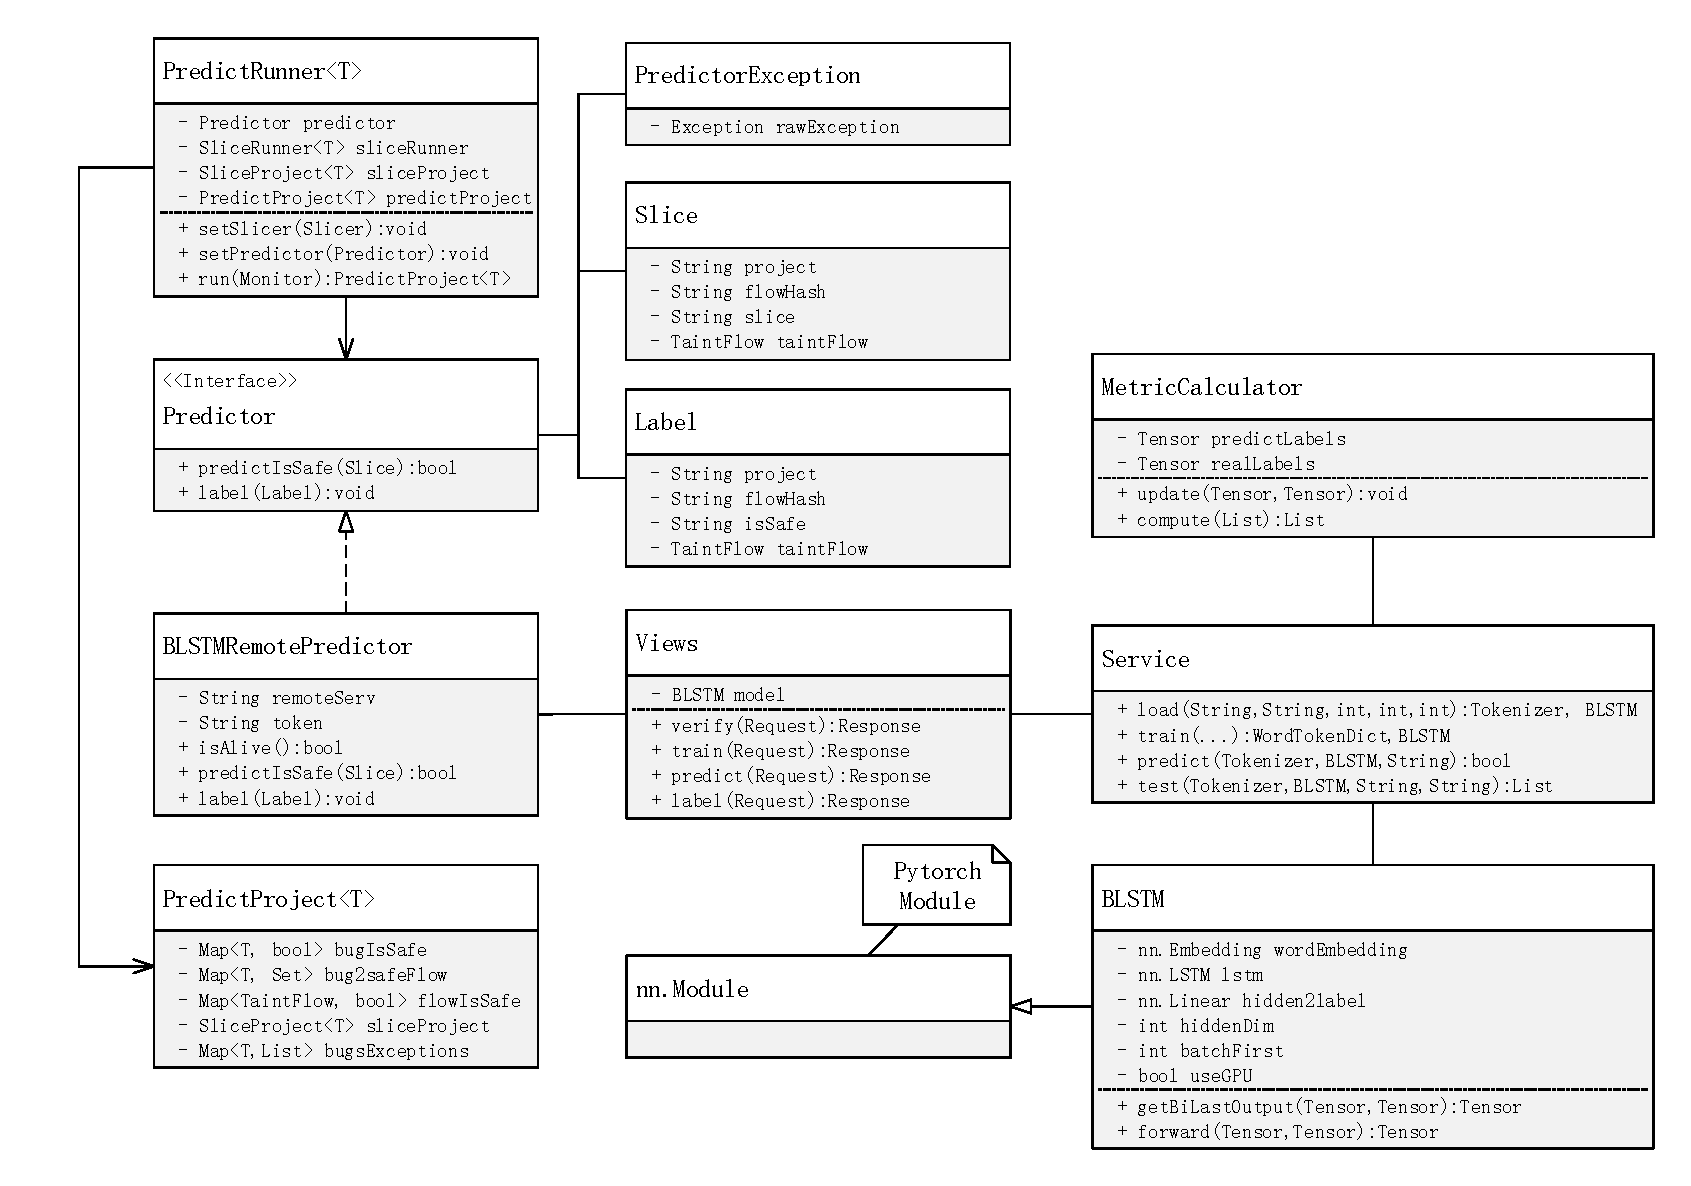
\includegraphics[width=0.9\linewidth]{FIGs/chapter3/predictClass.pdf}
    \caption{预测模块类图}\label{predictClass}
\end{figure}

预测器控制类用于对一个漏洞报告项目进行预测,其 predictor 属性是其预测的预测器实例,sliceRunner 是生成切片项目的控制器,sliceProject 保存切片模块的切片项目,predictProject 保存最终预测项目,其有设置切片器的方法 \textit{setSlicer()} 和设置预测器的方法 \textit{setPredictor()},进行预测的方法为 \textit{run()},预测进行前,若类中无切片项目,则会自动调用切片模块对其切片,接着再进行预测,最终方法返回预测结果。

PredictProject 类为预测结果项目类,包含最终预测结果,其属性 bugIsSafe 为漏洞实例至漏洞是否为误报的映射表(若漏洞安全则说明误报),bug2safeFlow 记录了漏洞至安全流的映射,用于向开发者解释污点消失于那些污染流,flowIsSafe 记录了单条污染流是否为误报,sliceProject为切片模块的项目,bugsExceptions 记录预测运行时发生的异常。

预测器接口 Predictor 用于实现漏洞预测控制和切片预测本身逻辑的解耦,其有两个方法:\textit{predictIsSafe()} 用于对一个切片进行预测,返回该切片是否是安全的,若切片安全,则说明污点在该污点流上无法传播,\textit{label()} 用于对切片进行标记。Slice 类和 Label 类分别对应以上两种方法的输入对象,Slice 类除了包含切片内容以外,还包括污染流对象,污染流哈希和项目名,Label 类包括了污染流对象,污染流哈希、项目名以及该污染流是否安全的标记。预测器在预测时允许抛出 PredictorException 异常,该异常类汇总含原始异常信息,以便错误跟踪。

BLSTMRemotePredictor 实现了预测器接口,其属性 remoteServ 记录服务器地址,token 记录身份令牌,除了实现接口方法外,其还有 \textit{isAlive()} 方法用于判断到远程服务器的连接是否有效。

Views 是远程服务器的对外服务类,其包含了验证口令是否合法的方法 verify()(对应于 BLSTMRemotePredictor.isAlive(),处理训练请求的方法 \textit{train()},处理预测请求的方法 \textit{predict()},以及处理标记请求的方法 \textit{label()},其 model 属性代表当前最新的模型实例。

Service 是模型的服务类,视图层接受到请求后,会将请求参数取出交给该类,再由该类调用 BLSTM 模型提供相应服务。这些服务主要有: \textit{load()} 用于加载一模型,其参数分为别为字典序列化文件的地址、BLSTM 序列化文件的地址、最小词频、词嵌入向量维度和隐藏层神经元个数; \textit{train()} 用于训练一个 BLSTM 模型,由于其参数较多这里省略,详细可以参照下一章中的表~\ref{sql:modelConfigTable}; \textit{predict()} 对应预测请求,其参数分别为序列化器、BLSTM 模型,以及一个切片字符串,返回该切片是否是安全的。\textit{test()} 用于测试一个神经网络模型准确率,前两个参数与 \textit{predict()} 方法相同,后面两个 String 类型参数分别为切片数据文件夹和标记数据文件夹。

MetricCalculator 为度量计算器类,其通过一系列度量指标用于评估预测效果,其属性 predictLabels 代表预测的标签,realLabels 为真实标签,\textit{update()} 方法用于增加预测和真实标签数据,\textit{compute()} 方法用于产生一系列度量值,其输入为一系列度量方法的名称,输出为这些度量的具体值。

BLSTM 类是 BLSTM 神经网络类,其继承于 pytorch 模型基类 nn.Module,本模块的神经网络有三层组成,首先是词嵌入层,对应属性为 wordEmbedding,其作用是将一个单词序号转换为一维向量,这样一组单词序列就可以转化为二维向量数据,接着是 BLSTM 层,对应属性为 lstm,nn.LSTM 为 pytorch 对象,模块只需将其指定属性指定为双向即可,最后为一个线性层 hidden2Label,该层用于将 BLSTM 输出映射到 0$\sim$1 的范围上。hiddenDim 记录隐藏层神经元数目,batchFirst 记录批量训练时的二维向量中,单条数据是以行向量形式给出($batchFirst=true$)还是列向量形式给出($batchFirst=false$),useGPU 指模型计算时是否需要用 GPU,这三个属性均需要在建立模型时给出。\textit{forward()} 方法为神经网络后向传播方法,其参数依次表示批量数据的二维向量,以及数据长度向量,返回预测结果,其会调用 \textit{getBiLastOutput()} 方法,该方法用于获取两个方向上的 LSTM 最后一个时刻的输出。\\

\subsection{流程设计}

本模块流程图如图~\ref{predictProcessing} 所示,本模块以切片模块的报告为输入,输出漏洞预测项目,其中记录每个漏洞是否为误报的预测结果。

\begin{figure}[!htbp]
    \centering
    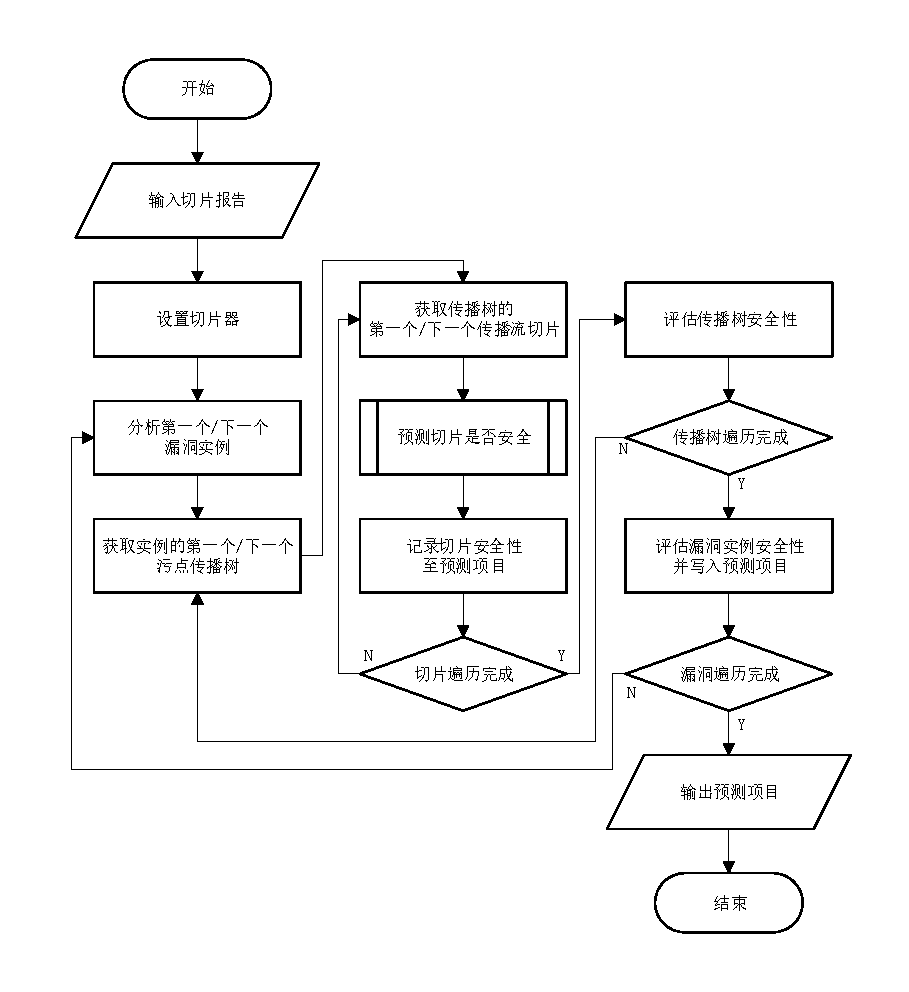
\includegraphics[width=0.9\linewidth]{FIGs/chapter3/predictProcessing.pdf}
    \caption{预测模块流程}\label{predictProcessing}
\end{figure}

模块首先初始化并设置一个切片器实例,随即处理每一个漏洞实例,对于单个漏洞实例,漏洞传播模块已经将其分解为了若干棵污点传播树,于是模块开始遍历这些传播树,对于每一个传播树,程序切片模块又已将其分解为若干条程序切片,因此模块将依次预测这些切片,并记录切片安全性,当切片遍历完成后,根据切片结果评估传播树的安全性,根据污点传播规则,只要有传播树上的一条传播流是安全的,那么整个传播树即为安全,接着当一漏洞的传播树遍历完成后,可以根据传播树的安全性评估漏洞是否为误报,根据漏洞触发规则,只要有一棵传播树是不安全的,那么漏洞即是真实的,否则为误报,将每个漏洞实例预测完后,模块输出预测项目结果。

本模块是系统中最后一个模块,也就是说,预测项目是本系统的最终输出,用户可以优先关注真实漏洞并展开修复工作,接着再观察误报漏洞是否为漏报,并对它们进行标记。

\section{数据库设计}
本系统的数据库主要用来存储用户身份信息、污点分析得到的污染流数据和标记、用于模型训练的参数配置信息以及模型本身信息。经过分类,可以总结为三类数据表:

第一类是与鉴权有关的数据表,由于本系统主要使用了C/S架构,为了防止恶意攻击者向服务器注入垃圾数据影响预测,因此需要对客户端身份进行鉴定,为此设立客户端口令(Client\_Token)表,由安全运营人员进行维护。

第二类是与程序分析相关的数据表,由于本系统后台主要是对子污染流的切片进行有监督预测,因此自然需要污染流(Taint\_Flow)表和对污染流的标记(Label)表,对一个污染流而言,需要对其函数入口和关注点(即语句位置)进行切片,因此存在函数摘要(Method\_Description)表和语句位置(Location)表,不同项目可能具有名称相同的类、函数或文件,为了在逻辑上唯一标识一个函数摘要和语句位置,因此建立项目(Project)表。

第三类是与模型本身相关的数据表,本系统使用BLSTM进行切片预测,对BLSTM训练和BLSTM结构本身涉及到一系列参数,为此将其保存在模型配置(Model\_Config)表中,供安全运营人员调整,对于已经训练好的模型,将其保存在BLSTM模型(LSTM\_Model)表中。

与鉴权有关的数据表实体关系图如图~\ref{er:token} 所示,其中只有一张表,即客户端口令表,其中字段如表~\ref{sql:tokenTable} 所示,id 为一个口令的唯一标识;token 为一字符串,由管理员设置和发放,客户端连接时需要有一合法 token 才可与服务器通信;description 用于保存该口令的一些描述信息;create\_time 为该口令的创建时间。

\begin{figure}[!htbp]
	\centering
	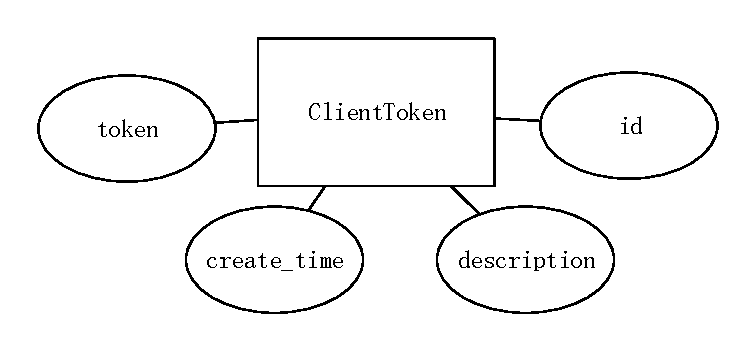
\includegraphics[width=0.5\linewidth]{FIGs/chapter3/token_er.pdf}
	\caption{与鉴权相关表的实体关系图}\label{er:token}
\end{figure}

\begin{table}[!htbp]\footnotesize %token table
	\centering
	\caption{Client\_Token 表}
	\vspace{2mm}
	% l - left, r - right, c - center. | means one vertical line 这里声明的是表格单元中的内容如何对齐
	\begin{tabular}{L{2cm}L{2cm}L{2.6cm}L{6cm}}
		\toprule
		\textbf{字段名}&\textbf{数据类型}&\textbf{属性}&\textbf{说明}\\
		\midrule
		id					&INT&PK&主键,token的唯一标识\\
		token 				&VARCHAR(255)&NN, UNIQUE&表示管理员向用户发放的 token\\
		description				 &VARCHAR(255)& N &用于保存管理员对此 token 的备注信息\\
		create\_time		  &DATETIME&NN&表示 token 的创建时间\\
		\bottomrule
	\end{tabular}
	\label{sql:tokenTable}
\end{table}

与程序分析相关的实体关系图如图~\ref{er:program},其中,项目表保存项目名称,函数摘要表保存一个项目中的函数摘要信息,语句位置表记录关注点所在的代码位置,污染流表记录污染流和其中的切片信息,标记表记录一个污染流记录是否是安全的。一个项目可以有多个函数摘要、位置和污染流,即有一对多的关系,一个函数摘要或语句位置可以有多个污染流记录,而标记和污染流记录呈一对一关系。

\begin{figure}[!htbp]
	\centering
	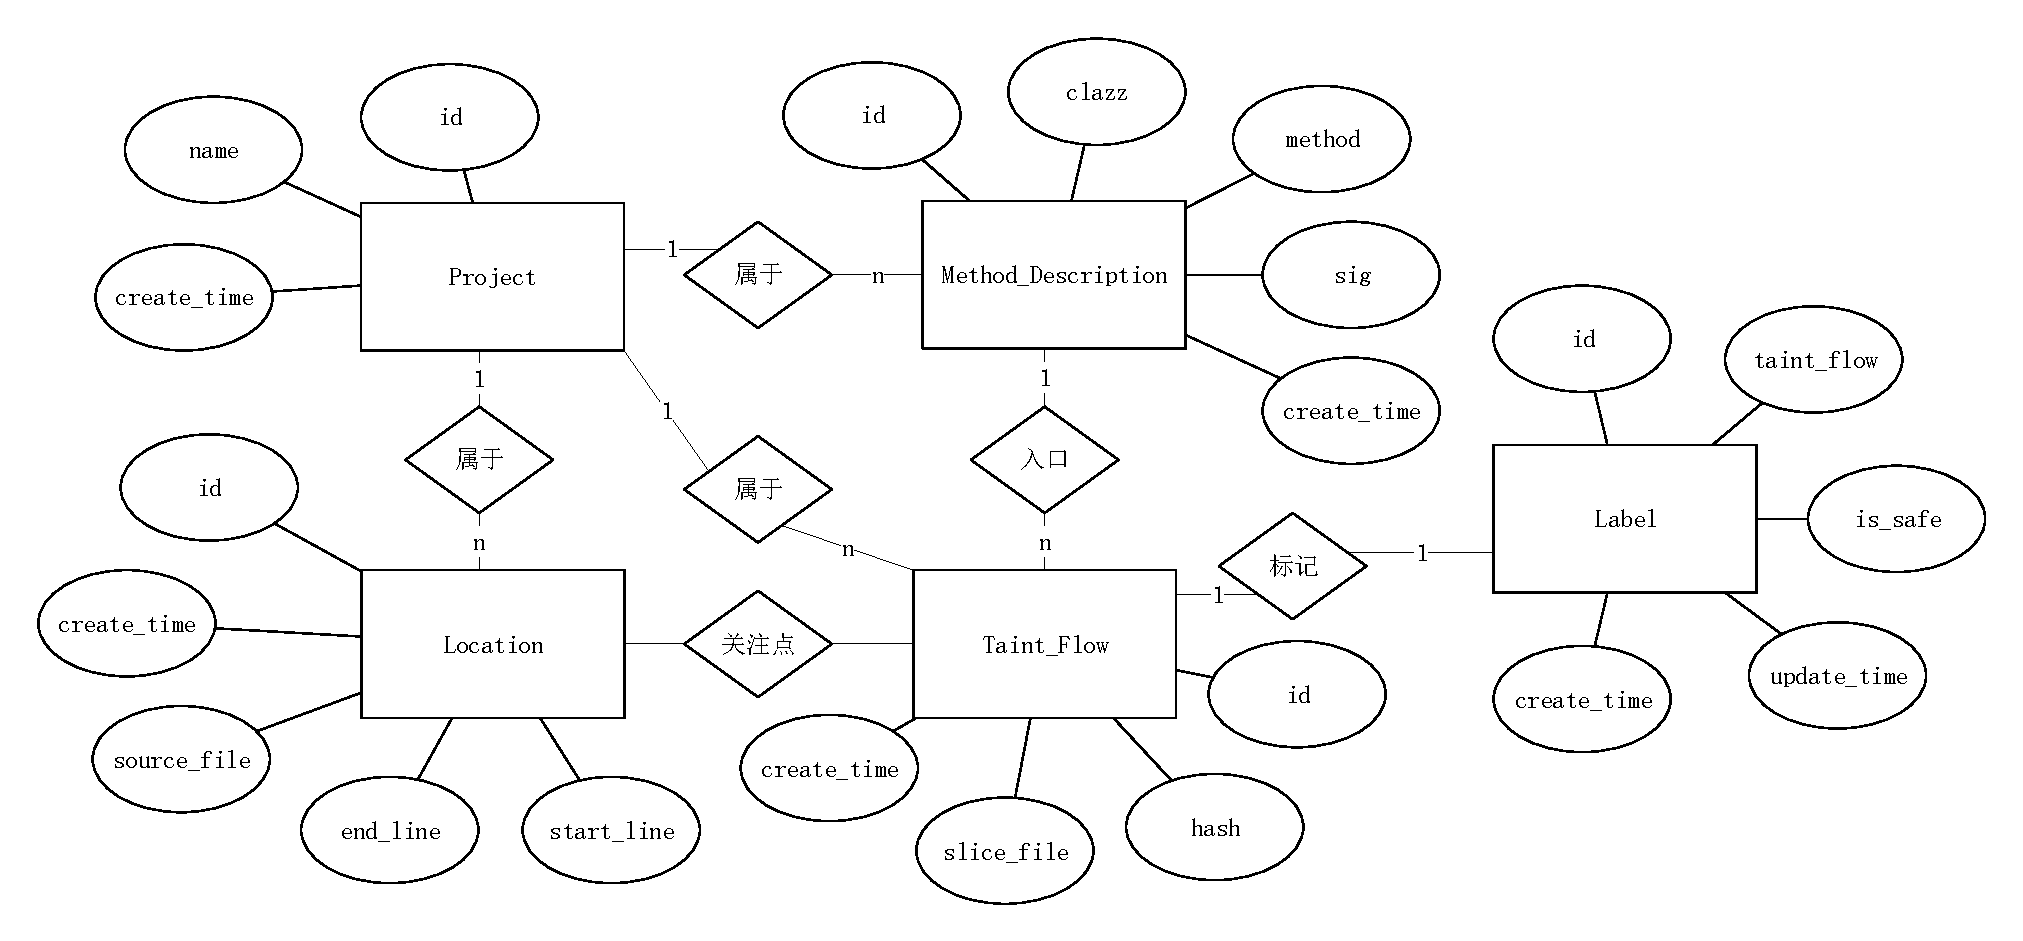
\includegraphics[width=1\linewidth]{FIGs/chapter3/program_er.pdf}
	\caption{与程序分析相关表的实体关系图}\label{er:program}
\end{figure}

表~\ref{sql:project}是对项目表的字段说明,其中,id是一个项目的唯一标识;name标识项目名称,存在唯一性约束,由客户端建立扫描项目时指定;create\_time记录该项目的创建时间。

\begin{table}[!htbp]\footnotesize %project table
	\centering
	\caption{Project 表}
	\vspace{2mm}
	% l - left, r - right, c - center. | means one vertical line 这里声明的是表格单元中的内容如何对齐
	\begin{tabular}{L{2cm}L{2cm}L{2.6cm}L{6cm}}
		\toprule
		\textbf{字段名}&\textbf{数据类型}&\textbf{属性}&\textbf{说明}\\
		\midrule
		id							&INT&PK&主键,项目的唯一标识\\
		name		 			&VARCHAR(255)&NN&表示项目的名称\\
		create\_time		  &DATETIME&NN&表示项目创建时间\\
		\bottomrule
	\end{tabular}
	\label{sql:project}
\end{table}

表~\ref{sql:methodDescription}是对函数摘要表的字段说明,其中,id 是一个函数摘要的唯一标识;clazz 记录函数的类名;method 记录函数的方法名;sig 记录函数签名,其包括了参数类型和返回值类型;project 作为外键,标识该函数摘要位于哪个项目中;create\_time记录该函数摘要的创建时间。此外,clazz,method,sig,project能够唯一标识一个函数摘要。
\begin{table}[!htbp]\footnotesize %methodDescription table
	\centering
	\caption{Method\_Description 表}
	\vspace{2mm}
	% l - left, r - right, c - center. | means one vertical line 这里声明的是表格单元中的内容如何对齐
	\begin{tabular}{L{2cm}L{2cm}L{2.6cm}L{6cm}}
		\toprule
		\textbf{字段名}&\textbf{数据类型}&\textbf{属性}&\textbf{说明}\\
		\midrule
		id					&INT&PK&主键,函数摘要的唯一标识\\
		clazz				&VARCHAR(255)&NN&表示该函数的类名\\
		method 			& VARCHAR(255) &NN&表示该函数的方法名\\
		sig					&VARCHAR(255)&NN&表示该函数的签名,即函数参数和返回值类型\\
		project  		  &INT&FK, NN&外键,指向Project,表示该函数出现在此项目中\\
		create\_time  &DATETIME&NN&表示标记创建时间\\
		\bottomrule
	\end{tabular}
	\label{sql:methodDescription}
\end{table}

表~\ref{sql:location}是对语句位置表的字段说明,其中,id是一个语句位置的唯一标识;source\_file记录该语句所在的文件名	;start\_line记录该位置开始的代码行号;end\_line记录该位置结束的代码行号  ;project作为外键,记录该位置位于哪个项目中;create\_time记录该项目的创建时间。此外,source\_file,start\_line,end\_line,project联合可以唯一标识一个语句位置。
\begin{table}[!htbp]\footnotesize %location table
	\centering
	\caption{Location 表}
	\vspace{2mm}
	% l - left, r - right, c - center. | means one vertical line 这里声明的是表格单元中的内容如何对齐
	\begin{tabular}{L{2cm}L{2cm}L{2.6cm}L{6cm}}
		\toprule
		\textbf{字段名}&\textbf{数据类型}&\textbf{属性}&\textbf{说明}\\
		\midrule
		id							&INT&PK&主键,语句位置的唯一标识\\
		source\_file		 	&VARCHAR(255)&NN&表示语句所在文件名\\
		start\_line 			& INT &NN, UNSIGNED&表示语句所在的开始行号\\
		end\_line				&INT&NN, UNSIGNED&表示语句所在的结束行号\\
		project  			  &INT&FK, NN&外键,指向Project,表示该位置出现在此项目中\\
		create\_time		  &DATETIME&NN&表示标记创建时间\\
		\bottomrule
	\end{tabular}
	\label{sql:location}
\end{table}

表~\ref{sql:taintFlow} 是对污染流表的字段说明,其中,id 是一个污染流的唯一标识;hash	是这个污染流的哈希,通过切片文本的SHA1得到;slice\_file 切片文件在硬盘上的保存位置,当数据库中记录删除时,切片文件也应被删除;entry和point分别为切片的入口点和关注点 ;project作为外键,记录污染流存在于哪个项目中;create\_time记录该污染流的创建时间。此外,entry,point和project可以联合唯一标识一个污染流记录。

\begin{table}[!htbp]\footnotesize %taintFlow table
	\centering
	\caption{Taint\_Flow 表}
	\vspace{2mm}
	% l - left, r - right, c - center. | means one vertical line 这里声明的是表格单元中的内容如何对齐
	\begin{tabular}{L{2cm}L{2cm}L{2.6cm}L{6cm}}
		\toprule
		\textbf{字段名}&\textbf{数据类型}&\textbf{属性}&\textbf{说明}\\
		\midrule
		id					&INT&PK&主键,污染流的唯一标识\\
		hash				&VARCHAR(255)&NN&表示污染流的哈希\\
	    slice\_file			& VARCHAR(255) &NN&表示污染流切片的文件名\\
		entry				&INT&FK&外键,指向Method\_Description,表示污染流切片的入口\\
		point				&INT&FK&外键,指向Location,表示污染流切片的结束位置\\
		project  		  &INT&FK, NN&外键,指向Project,表示污染流所在的项目\\
		create\_time  &DATETIME&NN&表示污染流的创建时间\\
		\bottomrule
	\end{tabular}
	\label{sql:taintFlow}
\end{table}

表~\ref{sql:label}是对标记表的字段说明,其中,id 是一个标记的唯一标识;taint\_flow 作为外键,指这被标记的污染流对象,同时一个污染流同时只能有一个标记;entry和point分别为切片的入口点和关注点 ;is\_safe 标记了该污染流是安全/不安全的;create\_time记录该标记的创建时间;update\_time记录该标记的更新时间。

\begin{table}[!htbp]\footnotesize %label table
	\centering
	\caption{Label 表}
	\vspace{2mm}
	% l - left, r - right, c - center. | means one vertical line 这里声明的是表格单元中的内容如何对齐
	\begin{tabular}{L{2cm}L{2cm}L{2.6cm}L{6cm}}
		\toprule
		\textbf{字段名}&\textbf{数据类型}&\textbf{属性}&\textbf{说明}\\
		\midrule
		id							&INT&PK&主键,标记的唯一标识\\
		taint\_flow		 		&INT &FK, NN&外键,指向Taint\_Flow,表示本标记的污染流对象\\
		is\_safe 				& BOOLEAN &NN&表示这个污染流是安全的\\
		create\_time		  &DATETIME&NN&表示标记创建时间\\
		update\_time		&DATETIME&NN&表示标记更新时间\\
		\bottomrule
	\end{tabular}
	\label{sql:label}
\end{table}

与模型相关的实体关系图如图~\ref{er:model} 所示,其中,模型配置(Model\_Config)表记录模型配置信息,主要包括了配置名,模型训练相关信息和 LSTM 模型的参数等,LSTM 模型表(LSTM\_Model)记录以训练好的模型信息,主要信息有训练度量,模型保存位置等,一个配置可以训练多个模型。

\begin{figure}[!htbp]
	\centering
	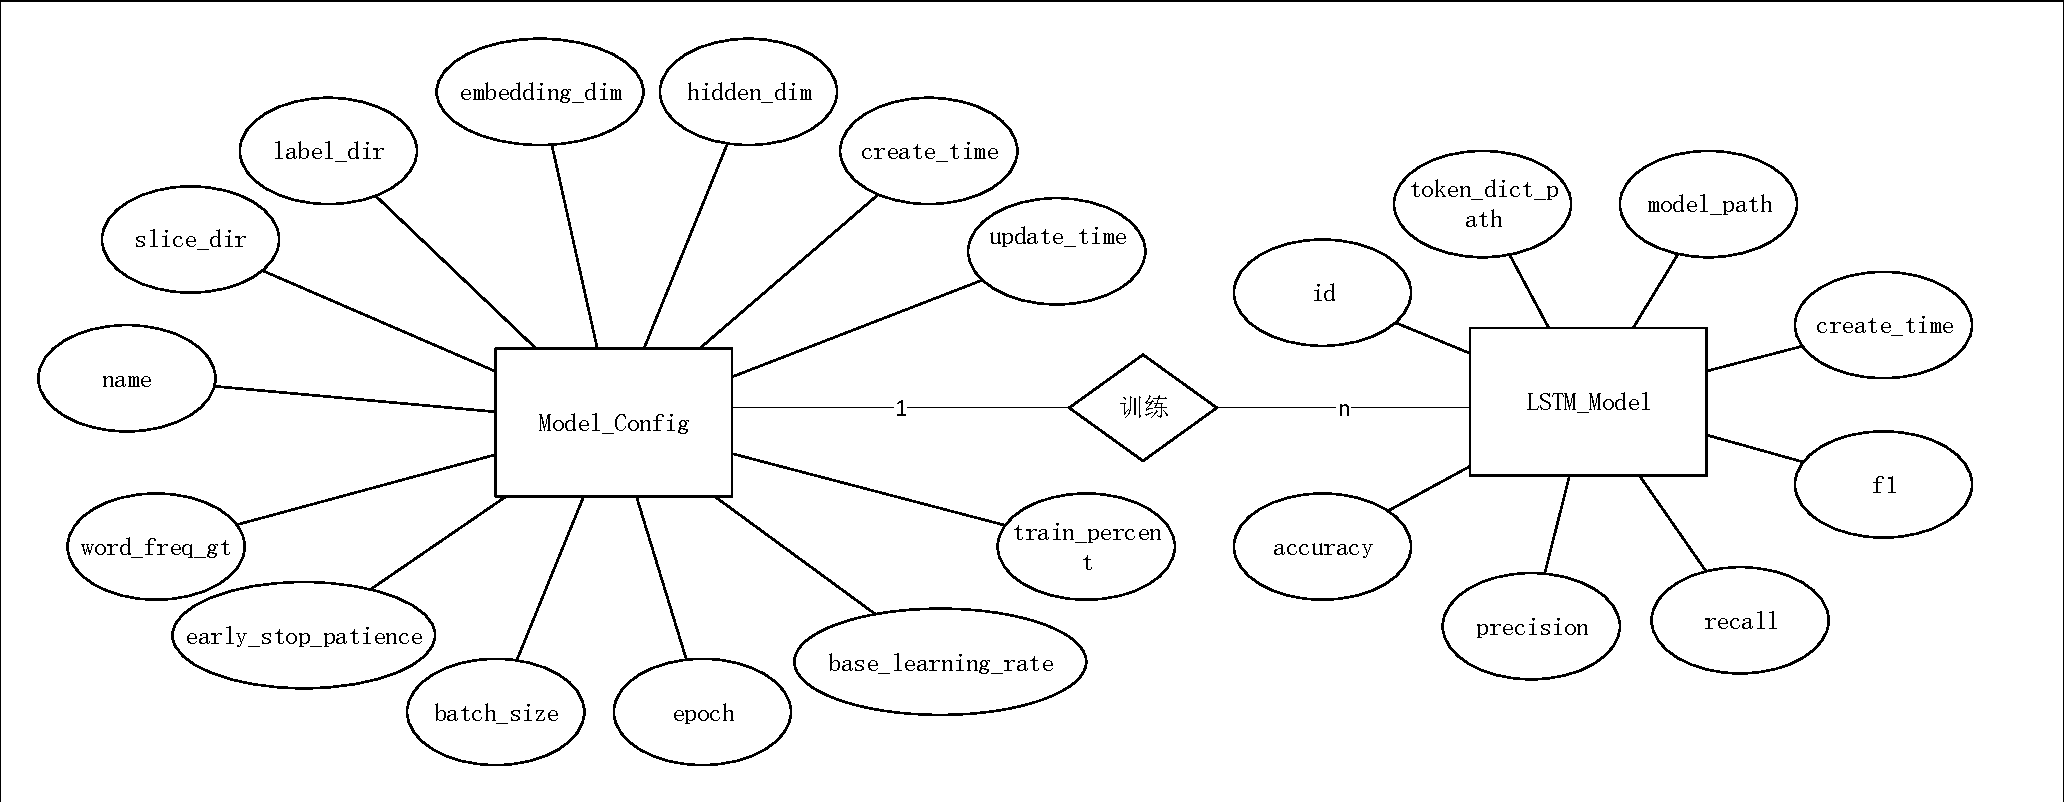
\includegraphics[width=1\linewidth]{FIGs/chapter3/model_er.pdf}
	\caption{与模型相关表的实体关系图}\label{er:model}
\end{figure}

 表~\ref{sql:modelConfigTable} 是对模型配置表的字段说明,其中 name 作为主键,用于唯一标识一个配置,训练时通过指定改值进行训练;slice\_dir 和 label\_dir 记录了学习用的数据集位置,分别表示了切片所在文件夹和标记所在文件夹(模型直接通过文件进行读取,而不从数据库读取,减少了IO消耗);embedding\_dim,hidden\_dim 为模型自身参数,分别代表词嵌入的维度和隐藏层神经元个数(模型的每层神经元个数相等);word\_freq\_gt 表示了将出现次数小于该值的单词表示为“UNK”(Unknown);early\_stop\_patience,base\_learning\_rate,batch\_size,epoch,train\_percent记录了模型训练的配置,early\_stop\_patience 值训练轮数超过改值后,若模型效果(loss)仍比之前最优效果差,则提前停止训练,base\_learning\_rate 指初始学习率,batch\_size 指批量传入模型的数据量,epoch 指最大训练轮数,train\_percent 指训练集占总数据集的百分比,剩下的数据作为训练集,用于评估训练效果;最后,create\_time 和 update\_time 分别表示配置创建时间和配置更新时间。

\begin{table}[!htbp]\footnotesize %model config table
	\centering
	\caption{Model\_Config 表}
	\vspace{2mm}
	% l - left, r - right, c - center. | means one vertical line 这里声明的是表格单元中的内容如何对齐
	\begin{tabular}{L{2.2cm}L{2cm}L{2.6cm}L{6cm}}
		\toprule
		\textbf{字段名}&\textbf{数据类型}&\textbf{属性}&\textbf{说明}\\
		\midrule
		name 						&VARCHAR(255)&PK&主键,唯一标识一个配置\\
		slice\_dir		 			&VARCHAR(255)&NN&模型使用切片数据所在的文件夹\\
		label\_dir		 			&VARCHAR(255)&NN&模型使用标记数据所在的文件夹\\
		embedding\_dim		  &INT&NN, UNSIGNED&词嵌入时的维度,值为正整数\\
		hidden\_dim				&INT&NN, UNSIGNED&隐藏层神经元的个数,值为正整数\\
		word\_freq\_gt			&INT&NN, UNSIGNED&最小词频,小于该词频则表示为UNK,值为正整数\\
		early\_stop\_patience		&INT&NN, UNSIGNED&提前停止忍耐度,如果学习轮数大于此值,效果仍比以前差则学习停止,值为正整数\\
		base\_learning\_rate		&DOUBLE&NN, UNSIGNED&初始学习率\\
		batch\_size					&INT&NN, UNSIGNED&批量数据记录数,每次向神经网络输入batch\_size条记录,再进行反向传播\\
		epoch						&INT&NN, UNSIGNED&训练最大迭代次数,超过该次数则停止训练\\
		train\_percent						&DOUBLE&NN, UNSIGNED&表示训练集占整个数据的百分比,默认为1,即将所有数据代入训练\\
		create\_time				&INT&NN, UNSIGNED&配置创建时间\\
		update\_time				&INT&NN, UNSIGNED&配置更新时间\\
		\bottomrule
	\end{tabular}
	\label{sql:modelConfigTable}
\end{table}

表~\ref{sql:lstmModelTable} 是对 BLSTM 模型表的字段说明,其中 id 作为主键唯一标识一个模型;token\_dict\_path 和 model\_path 分别表示单词到整形值的映射字典文件位置和BLSTM模型位置,这两个字段用于加载模型实现对切片的预测;config 表示模型是由何配置训练得到的;accuracy、precision、recall和F1表示了模型的四种度量,当配置划分没有训练集时,这些值为-1;create\_time记录模型被训练出的时间。

\begin{table}[!htbp]\footnotesize %lstm model table
	\centering
	\caption{BLSTM\_Model表}
	\vspace{2mm}
	% l - left, r - right, c - center. | means one vertical line 这里声明的是表格单元中的内容如何对齐
	\begin{tabular}{llll}
		\toprule
		\textbf{字段名}&\textbf{数据类型}&\textbf{属性}&\textbf{说明}\\
		\midrule
		id&INTEGER&PK&主键,模型的唯一标识\\
		token\_dict\_path &VARCHAR(255)&NN&保存单词到tokenid的字典文件位置\\
		model\_path		 &VARCHAR(255)&NN&保存BLSTM模型文件的位置\\
		config				 &VARCHAR(255)&FK,NN&指向Model\_Config表,表示模型对应的配置信息\\
		accuracy	&DOUBLE&NN&表示学习后训练集的准确率,若无训练集则为-1\\
		precision	&DOUBLE&NN&表示学习后训练集的精确率,若无训练集则为-1\\
		recall	&DOUBLE&NN&表示学习后训练集的召回率,若无训练集则为-1\\
		F1	&DOUBLE&NN&表示学习后训练集的F1,若无训练集则为-1\\
		create\_time		  &TIME&NN&记录模型创建时间\\
		\bottomrule
	\end{tabular}
	\label{sql:lstmModelTable}
\end{table}

\section{本章小结}